\documentclass{article}
\usepackage{JASA_manu} %formats document like ASA wants
\usepackage{jasa_harvard} %formats citations like ASA wants
\usepackage{amssymb, amsmath, amsthm, graphics, graphicx, color, fullpage}
\usepackage{thmtools} %to format the Algorithm environment correctly
\usepackage{nameref, hyperref, cleveref} %for named references
\usepackage{zref-xr, zref-user} %for hyperlinked references to outside docs
\zexternaldocument*{dlmasisapp} %supplementary materials
%use \zref{label} to reference items there

% define algorithm environment
\declaretheoremstyle[
notefont=\bfseries, notebraces={}{},
bodyfont=\normalfont\itshape,
headformat=\NAME:\NOTE
]{nopar}
\declaretheorem[style=nopar, name=Algorithm, 
refname={Algorithm,Algorithms},
Refname={Algorithm,Algoritms},
numbered=no]{alg*}

\newtheorem{thm}{Theorem}[subsection]
\newtheorem{prop}[thm]{Proposition}
\newtheorem{cor}[thm]{Corollary}
\newtheorem{lem}[thm]{Lemma}

\DeclareMathOperator{\tr}{tr}
\DeclareMathOperator{\B}{B}
\DeclareMathOperator{\vech}{vech}
\DeclareMathOperator{\vect}{vec}

\graphicspath{{plots/}}
\newcommand{\matt}[1]{{\color{red} Matt: #1}}
\newcommand{\jarad}[1]{{\color{red} Jarad: #1}}

\usepackage[page,header]{appendix}
\usepackage{titletoc}


\begin{document}


\title{Interweaving Markov chain Monte Carlo strategies for efficient
estimation of dynamic linear models}
\author{Matt Simpson, Jarad Niemi, Vivekananda Roy}
\date{\today}
\maketitle

\begin{abstract}
In dynamic linear models (DLMs) with unknown fixed parameters and latent states, a common Markov chain Monte Carlo (MCMC) sampling strategy is to alternate sampling of latent states conditional on fixed parameters and sampling of fixed parameters conditional on latent states. In some regions of the parameter space, this standard data augmentation (DA) algorithm can be inefficient. To improve efficiency, we seek to employ the interweaving strategies of \citeasnoun{yu2011center} that combine separate DAs by weaving them together. Toward this end, we introduce a number of novel alternative DAs for a general class of DLMs: scaled errors, scaled disturbances, wrongly-scaled errors, and wrongly-scaled disturbances. Each DA implies a unique MCMC sampling strategy and these strategies can be more or less efficient across the parameter space. Interweaving these strategies results in 


One of these strategies, ancillary-sufficient interweaving strategy (ASIS) requires one the two DAs to be a sufficient augmentation and the other to be an ancillary augmentation, also known as centered and noncenterd augmentations respectively. We show, however, that under reasonable assumptions any sufficient augmentation requires sampling from a density that is just as complicated as the target posterior distribution. Nonetheless, we utilize  augmentations to construct several interweaving algorithms -- both the standard general interweaving strategy (GIS), of which ASIS is a subspecies, and the componentwise interweaving strategy (CIS) which applies GIS to sub-blocks of the parameter vector in a Gibbs-like structure. Though we cannot construct an ASIS algorithm, we are able to construct a CIS algorithm that uses ASIS in each parameter block. Using the local level DLM, we show how to construct several of these algorithms and conduct a simulation study in order to discern their properties. We find several algorithms that outperform the standard DA for many regions of the parameter space.
\end{abstract}


\section{Variations of data augmentation}\label{sec:Intro}

Ever since the seminal paper by \citeasnoun{tanner1987calculation}, data augmentation has become a common strategy for constructing MCMC algorithms to sample from intractable probability distributions. Suppose $p(\phi|y)$ is the target density, in this case the posterior distribution of some parameter $\phi$ given data $y$. We use $p(.)$ to denote the probability density of the enclosed random variables. Then the data augmentation (DA) algorithm adds a data augmentation $\theta$ with joint distribution $p(\phi,\theta|y)$ such that $\int_{\Theta}p(\phi,\theta|y)d\theta = p(\phi|y)$. The DA algorithm is similar to a Gibbs sampler, except it constructs a Markov chain for $\phi$ instead of $(\phi, \theta)$. In the DA algorithm, the $k+1$'st state of $\phi$ is obtained from the $k$'th state as follows (we implicitly condition on the data $y$ in all algorithms and only superscript the previous and new draws of the model parameters of interest):
\begin{alg*}[DA]Data Augmentation\label{alg:DA}
  \begin{align*}
  [\theta|\phi^{(k)}] \to [\phi^{(k+1)}|\theta]
\end{align*}
\end{alg*} 
\noindent Here $[\theta|\phi^{(k)}]$ means a draw of $\theta$ from $p(\theta|\phi^{(k)},y)$ and $[\phi^{(k+1)}|\theta]$ means a draw from $p(\phi|\theta,y)$. The DA, $\theta$, need not be interesting in any scientific sense --- it can be viewed purely as a computational construct. However for cases where the DA is intrinsically interesting, the DA algorithm does incidentally obtain joint draws from $p(\phi,\theta|y)$ and in that sense can be viewed as a Gibbs sampler. For our purposes, $\theta$ is a nuisance parameter.

The EM algorithm of \citeasnoun{dempster1977maximum} and its variants are closely analogous to DA algorithms --- specifically the DA algorithm can be viewed as a stochastic version of the EM algorithm. In fact there is a long history of using methods typically used to speed up convergence of the EM algorithm to construct alternatives to DA that converge faster and vice versa; \citeasnoun{van2010cross} shows how much overlap in the two literatures exists. The main advantage of DA and EM algorithms is their ease of implementation, but much of this work is necessary because DA and EM algorithms can often be prohibitively slow. 

\subsection{Reparameterization and alternating DAs}

One well known method of improving mixing and convergence in MCMC samplers and convergence in the EM algorithm is reparameterizing the model. Most of the literature in some way focuses on what are called centered and noncentered parameterizations. See for example \citeasnoun{papaspiliopoulos2007general} who provide a good summary of these methods. In our notation where $\phi$ is the parameter, $\theta$ is the DA and $y$ is the data, the parameterization $(\phi,\theta)$ is a {\it centered parameterization} (CP) if $p(y|\theta,\phi)=p(y|\theta)$. The parameterization is a {\it noncentered parameterization} (NCP) if $p(\theta|\phi)=p(\theta)$. When $(\phi,\theta)$ is a CP, $\theta$ is called a {\it centered augmentation} (CA) for $\phi$ and when $(\phi,\theta)$ is a NCP, $\theta$ is called a {\it noncentered augmentation} (NCA) for $\phi$. A CA is sometimes called a {\it sufficient augmentation} (SA) and a NCA is sometimes called an {\it ancillary augmentation} (AA)\cite{yu2011center}. Like \citeasnoun{yu2011center}, we prefer the latter terminology because it immediately suggests the intuition that an SA is like a sufficient statistic while an AA is like an ancillary statistic and hence Basu's theorem suggests that they are conditionally independent given $\phi$ \cite{basu1955statistics}. 

The key reasoning behind the emphasis on SAs and AAs is that typically when the DA algorithm based on the SA has nice mixing and convergence properties, the DA algorithm based on the AA has poor mixing and convergence properties and vice-versa. This property suggests that there might be a way to combine the two such DA algorithms or the two underlying parameterizations in order to construct an improved sampler. Some work focuses on using partially noncentered parameterizations that are a sort of bridge between the CP and NCP, for example \citeasnoun{papaspiliopoulos2007general} consider such parameterizations for general hierarchical models and \citeasnoun{fruhwirth2004efficient} in the context of a particular DLM --- a dynamic univariate regression with a stationary AR(1) coefficient. Another suggestion by \citeasnoun{papaspiliopoulos2007general} is to alternate between the two augmentations within a Gibbs sampler. Suppose we have a second distinct DA $\gamma$ such that $\int_\Gamma p(\phi,\gamma|y)d\gamma = p(\phi|y)$. Then the {\it alternating} algorithm for sampling from $p(\phi|y)$ is as follows:
\begin{alg*}[Alt]Alternating Algorithm\label{alg:Alt} 
  \begin{center}
    \begin{tabular}{lllllll}
  $[\theta|\phi^{(k)}]$& $\to$& $[\phi|\theta]$& $\to$& $[\gamma|\phi]$& $\to$& $[\phi^{(k+1)}|\gamma]$
    \end{tabular}
  \end{center}
\end{alg*}
\noindent One iteration of the alternating algorithm consists of one iteration of the DA algorithm based on $\theta$ to obtain an intermediate value of $\phi$, followed by one iteration of the DA algorithm based on $\gamma$ started at the intermediate value of $\phi$. 

Recall that a typical problem with slow MCMC is that there is high autocorrelation in the Markov chain for $\phi$, $\{\phi^{(k)}\}_{k=1}^K$, leading to imprecise estimates of $\mathrm{E}[f(\phi)|y]$, the expectation of some function $f$ with respect to the posterior density of $\phi$. Our goal is to reduce this dependence. In Algorithm \nameref{alg:DA}, when $\phi$ and $\theta$ are highly dependent in the joint posterior, the draws from $p(\theta|\phi,y)$ and then from $p(\phi|\theta,y)$ will hardly move the chain, resulting in high autocorrelation. In an alternating algorithm, there are essentially two chances to substantially move the chain -- one for $\theta$ in the draws from $p(\theta|\phi,y)$ and from $p(\phi|\theta,y)$ and one for $\gamma$ in the draws from $p(\gamma|\phi,y)$ and from $p(\phi|\gamma,y)$.  In particular, when $\theta$ is an SA and $\gamma$ is an AA or vice versa, then it is often the case that there is low dependence either between $\phi$ and $\theta$ or between $\phi$ and $\gamma$. As a result, either steps 1 and 2 or steps 3 and 4 will substantially move the chain in the alternating algorithm, which limits how poorly the algorithm can perform.

\subsection{Interweaving: an alternative to alternating}\label{sec:Intro:int}

One recent advance that is similar to an alternating strategy is the notion of {\it interweaving} the two DAs together \cite{yu2011center}. Under the conditions required for the alternating algorithm a general interweaving strategy (GIS) is an MCMC algorithm that obtains $\phi^{(k+1)}$ from $\phi^{(k)}$ as follows:
\begin{alg*}[GIS]General Interweaving Strategy\label{alg:GIS}
  \begin{align*}
    [\theta|\phi^{(k)}] \to [\gamma|\theta] \to [\phi^{(k+1)}|\gamma].
  \end{align*}
\end{alg*}
\noindent The GIS algorithm obtains the $k+1$st iteration of the parameter vector $\phi$ from the $k$th iteration in three steps. First, it draws the DA $\theta$ conditional on $\phi^{(k)}$ (and the data). Next, it draws the DA $\gamma$ conditional on $\theta$. Finally, it draws $\phi^{(k+1)}$ conditional on $\gamma$. This looks similar to the usual DA algorithm, except a second DA is ``weaved'' in between the draw of the first DA and of the parameter vector. Step two of the GIS algorithm is typically accomplished by sampling $\phi|\theta,y$ and then $\gamma|\theta,\phi,y$. In addition, $\gamma$ and $\theta$ are often, but not always, one-to-one transformations of each other conditional on $(\phi,y)$, i.e. $\gamma = M(\theta;\phi,y)$ where $M(.;\phi,y)$ is a one-to-one function. If we expand out step two, then the algorithm becomes:
\begin{alg*}[GIS-E]Expanded GIS\label{alg:GIS2}
  \begin{center}
    \begin{tabular}{lllllll}
      $[\theta|\phi^{(k)}]$& $\to$& $[\phi|\theta]$& $\to $&$[\gamma|\theta,\phi]$& $\to$& $[\phi^{(k+1)}|\gamma]$
    \end{tabular}
  \end{center}
\noindent \end{alg*}
When $\gamma$ is a one-to-one transformation of $\theta$, step three is simply a transformation from $\theta$ to $\gamma$, i.e. $\gamma=M(\theta;\phi,y)$. The key difference between Algorithm \nameref{alg:GIS} and Algorithm \nameref{alg:Alt} can be seen in step three of the expanded version of GIS, Algorithm \nameref{alg:GIS2}. Instead of drawing from $p(\gamma|\phi,y)$, the GIS algorithm draws from $p(\gamma|\theta,\phi,y)$, connecting the two DAs together while the alternating algorithm keeps them separate.

\citeasnoun{yu2011center} call a GIS approach where one of the DAs is an SA and the other is an AA an {\it ancillary sufficient interweaving strategy}, or an ASIS. They show that the GIS algorithm has a geometric rate of convergence no worse than the worst of the two underlying DA algorithms and in some cases better than the the corresponding alternating algorithm. In particular, their Theorem 1 suggests that the weaker the dependence between the two data augumentations in the posterior, the more efficient the GIS algorithm. With a posteriori independent data augmentations, the GIS algorithm will even obtain iid draws from the posterior density of the model parameter. This helps motivate their focus on ASIS --- conditional on the model parameter, an SA and an AA are independent under the conditions of Basu's theorem \cite{basu1955statistics}, which suggests that the dependence between the two DAs will be limited in the posterior. In fact, when the prior on $\phi$ is nice in some sense, \citeasnoun{yu2011center} show that the ASIS algorithm is the same as the optimal parameter expanded data augmentation (PX-DA) algorithm of \citeasnoun{liu1999parameter}, which is closely related to marginal and conditional augmentation \cite{hobert2008theoretical,meng1999seeking}.

To gain some intuition about why interweaving works, we can first make a direct comparison between Algorithm \nameref{alg:Alt} and Algorithm \nameref{alg:GIS2}. Like the alternating algorithm, there are two opportunities for the Markov chain to move in the GIS algorithm, one each for $\theta$ and $\gamma$. So when the two underlying DA algorithms perform poorly in opposite regions of the parameter space, like, either steps 1 and 2 or steps 3 and 4 will substantially move the chain, limiting how poor Algorithm \nameref{alg:GIS} can perform -- much like Algorithm \nameref{alg:Alt}. However, \citeasnoun{yu2011center} show that the GIS algorithm is often much more efficient than the alternating algorithm. When the posterior dependence between the two DAs is low, step 2 in Algorithm \nameref{alg:GIS} (i.e. steps 2 and 3 in Algorithm \nameref{alg:GIS2}) is enough to almost completely break the dependence in the chain. For Algorithm \nameref{alg:Alt}, it is typically not feasible to find a data augmentation such that its step 2 or step 3 completely breaks the dependence in the chain --- this would require finding a DA such that the model parameter and the DA are essentially independent which, in turn, would likely mean that drawing from the conditional posterior of the parameter given the DA is nearly as difficult as drawing from the marginal posterior of the model parameter.

The particular method of interweaving discussed above is called a GIS or a {\it global} interweaving strategy since interweaving occurs globally across the entire parameter vector. It is possible to define a {\it componentwise} interweaving strategy (CIS) that interweaves within specific steps of a Gibbs sampler as well. A CIS algorithm for $\phi=(\phi_1, \phi_2)$ essentially employs interweaving for each block of $\phi$ separately, e.g.
\begin{alg*}[CIS]Componentwise Interweaving Strategy\label{alg:CIS}
  \begin{center}
    \begin{tabular}{llllll}
      $[\theta_1|\phi_1^{(k)},\phi_2^{(k)}]$ & $\to$  & $[\gamma_1|\phi_2^{(k)},\theta_1]$ & $\to$ & $[\phi_1^{(k+1)}|\phi_2^{(k)},\gamma_1]$ &$\to$ \\
      $[\theta_2|\phi_1^{(k+1)},\phi_2^{(k)},\gamma_1]$ &$\to$ & $[\gamma_2|\phi_1^{(k+1)},\theta_2]$ & $\to$ & $[\phi_2^{(k+1)}|\phi_1^{(k+1)},\gamma_2]$ &
    \end{tabular}
  \end{center}
\end{alg*}\noindent 
where $\theta_i$ and $\gamma_i$ are distinct data augmentations for $i=1$ and $i=2$, but potentially $\gamma_1=\theta_2$  or $\gamma_2=\theta_1$. The first line draws $\phi_1$ conditional on $\phi_2$ using interweaving in a Gibbs step, while the second line does the same for $\phi_2$ conditional on $\phi_1$. The algorithm can easily be extended to greater than two blocks within $\phi$. The main attraction of CIS is that it is often easier to find an AA--SA pair of DAs for $\phi_1$ conditional on $\phi_2$ and another pair for $\phi_2$ conditional on $\phi_1$ than it is to find and AA--SA pair for $\phi=(\phi_1,\phi_2)$ jointly. 

Most of the work on constructing and using DAs has focused on multilevel models --- e.g. \citeasnoun{van2001art} and \citeasnoun{papaspiliopoulos2007general}, but relatively little attention has been paid to time series models despite strong similarities between some time series models and the hierarchical models typically studied. We seek to improve DA schemes in a particular class of models --- linear, Gaussian statespace models, a.k.a. dynamic linear models (DLMs). Most of the existing literature focuses on non-Gaussian statespace models --- in particular the stochastic volatility model (see \citeasnoun{shephard1996statistical} for a summary), but few directly work with the class of DLMs we consider. In \citeasnoun{pitt1999analytic}, the authors analytically study convergence in the AR(1) plus noise model, but assume the observation and system variances are constant throughout. \citeasnoun{strickland2008parameterisation} considers reparameterization of the stochastic volatility and stochastic conditional duration models. \citeasnoun{fruhwirth2008heston} also consider reparameterizations of the stochastic volatility model while \citeasnoun{kastner2013ancillarity} applies ASIS in order to estimate the model. \citeasnoun{bos2006inference} consider a class of DLMs where the variances are time-dependent following a stochastic volatility process and show how a reparameterization can improve MCMC estimation. In the non-Gaussian Ornstein--Uhlenbeck stochastic volatility process, \citeasnoun{roberts2004bayesian} explores several alternate parameterizations and finds that the sampler based on the NCP always outperforms the sampler based on the CP. \citeasnoun{fruhwirth2003bayesian} directly applies several reparameterization techniques to a particular DLM -- a dynamic regression model with stationary AR(1) regression coefficient-- but focuses on estimation of the regression coefficient process.

The rest of the paper is organized as follows. In Section \ref{sec:DLM} we introduce the dynamic linear model, discuss the subclass of DLMs we consider, and explore some of the key properties of the model. Section \ref{sec:DAs} explores several possible DAs for our class of DLMs, including several new DAs, and shows that any SA for the DLM is likely to be difficult to use. Section \ref{sec:Algs} discusses the various MCMC strategies available for the DLM, including several DA algorithms, alternating algorithms, and interweaving algorithms. Section \ref{sec:LLM} applies these algorithms to a particular DLM --- the local level model --- and discusses some interesting problems which arise during the construction of these algorithms before using a simulation to empirically examine how well various algorithms perform across different regions of the parameter space. Finally, Section \ref{sec:Discuss} discusses these results and what they might mean for more general DLMs, provides an example to show how to extend some of the algorithms to a more general class of DLMs and suggests directions for further research.

\section{Dynamic linear models} \label{sec:DLM} 

The general dynamic linear model is well studied \cite{harrison1999bayesian,petris2009dynamic,prado2010time} and is defined as
\begin{align}
y_t &= F_t\theta_t + v_t && v_t \stackrel{ind}{\sim} N_k(0,V_t) && (\mbox{observation equation}) \label{dlmtdobseq}\\
 \theta_t &= G_t\theta_{t-1} + w_t && w_t \stackrel{ind}{\sim} N_p(0,W_t) && (\mbox{system equation}) \label{dlmtdsyseq}
\end{align}
where $N_d(\mu,\Sigma)$ is a $d$-dimensional multivariate normal distribution with mean $\mu$ and covariance $\Sigma$ and the observation errors, $v_{t}$ for $t=1,2,\cdots,T$, and system disturbances, $w_{t}$ for $t=1,2,\cdots,T$, are assumed independent. The observed data is $y\equiv y_{1:T} \equiv (y_1',y_2',\cdots y_T')'$ while $\theta \equiv \theta_{0:T} \equiv (\theta_0',\theta_1',\cdots \theta_T')'$ is called the latent states and is the usual DA for this model. For each $t=1,2,\cdots,T$, $F_t$ is a $k\times p$ matrix and $G_t$ is a $p\times p$ matrix. Let $\phi$ denote the vector of unknown parameters in the model. Then possibly $F_{t}$, $G_{t}$, $V_{t}$, and $W_{t}$ are all functions of $\phi$ for $t=1,2,\cdots,T$.

The subclass of DLMs we will focus on sets $V_t=V$ and $W_t=W$ and treats $F_{t}$ and $G_{t}$ as known for all $t$. Our results can be extended when $V_t$ or $W_t$ is time-varying or when $F_t$ or $G_t$ depend on unknown parameters, but we ignore those cases for simplicity. As a result $\phi=(V,W)$ is our unknown parameter vector and we can write the model as
\begin{align}
  y_t|\theta,V,W \stackrel{ind}{\sim} & N_k(F_t\theta_t,V) &
  \theta_t|\theta_{0:t-1},V,W  \sim & N_p(G_t\theta_{t-1},W) \label{dlmbotheqs}
\end{align}
for $t=1,2,\cdots T$. To complete the model specification in a Bayesian context, we need priors on $\theta_0$, $V$, and $W$. We will use the standard conditionally conjugate approach and assume that they are mutually independent a priori and that $\theta_0 \sim N_p(m_0, C_0)$, $V \sim IW(\Lambda_V, \lambda_V)$ and $W \sim IW(\Lambda_W, \lambda_W)$ where $m_0$, $C_0$, $\Lambda_V$, $\lambda_V$, $\Lambda_W$, and $\lambda_W$ are known hyperparameters and $IW(\Lambda, \lambda)$ denotes the inverse Wishart distribution with degrees of freedom $\lambda$ and positive definite scale matrix $\Lambda$. 

\subsection{The implied marginal model}\label{sec:DLM:marg}

While the DLM is typically defined using the latent states as a DA, strictly speaking they are unnecessary for the model's definition. Since we view $\theta$ purely as a nuisance parameter added for computational convenience, we wish to characterize the the marginal model for $y$ -- that is the model with $\theta$ integrated out. From equation \eqref{dlmbotheqs} we can rewrite the model by recursive substitution:
\begin{align*}
  y_t &= v_t + F_t\left(w_t + G_tw_{t-1} + G_tG_{t-1}w_{t-2} + ... + G_tG_{t-1}\cdots G_{2}w_1 + G_tG_{t-1}\cdots G_1\theta_0\right).
\end{align*}
Then conditional on $\phi=(V,W)$ each $y_t$ is a linear combination of normal random variables. After marginalizing out $\theta$, $y$ has a normal distribution such that $\mathrm{E}[y_t|\phi] =  F_tH_tm_0$,
\begin{align*}
  \mathrm{Var}[y_t|\phi] =  V + F_tK_tWK_t'F_t' + F_tH_tC_0H_t'F_t',\quad \mathrm{and} \quad
  \mathrm{Cov}[y_s,y_t|\phi] = F_sK_sWK_t'F_t' + F_sH_sC_0H_t'F_t',
\end{align*}
where $H_t = G_tG_{t-1}\cdots G_1$ and $K_t = I_p + G_t + G_tG_{t-1} + \cdots + G_tG_{t-1}\cdots G_2$. Next define $D_t = F_tG_tG_{t-1}\cdots G_1$. Then let
\begin{align*}
\tilde{V}_{Tk\times Tk} & = \begin{bmatrix} 
V & 0 & \ddots & 0\\
0 & V & \ddots & 0\\
\ddots & \ddots & \ddots & \ddots\\
0 & 0 & \ddots & V 
\end{bmatrix}, &
D_{Tp\times Tk} &= \begin{bmatrix} 
D_1 & 0 & \ddots & 0\\
0 & D_2 & \ddots & 0\\
\ddots & \ddots & \ddots & \ddots\\
0 & 0 & \ddots & D_T 
\end{bmatrix}, 
\end{align*}
\begin{align*}
\tilde{W}_{Tk\times Tk} &= \begin{bmatrix} K_1'F_1' & K_2'F_2' & \hdots K_T'F_T' \end{bmatrix}' W \begin{bmatrix} K_1'F_1' & K_2'F_2' & \hdots K_T'F_T' \end{bmatrix},&\\
\tilde{C}_{Tk\times Tk} &= \begin{bmatrix} H_1'F_1' & H_2'F_2' & \hdots H_T'F_T' \end{bmatrix}' C_0 \begin{bmatrix} H_1'F_1' & H_2'F_2' & \hdots H_T'F_T' \end{bmatrix},&
\end{align*} 
and $\tilde{m}_{Tp\times 1} = (m_0', m_0', \cdots m_0')'$. Now we have the data model for $y$ without any data augmentation:
\begin{align}
  y \stackrel{ind}{\sim} N_{Tk}(D\tilde{m}, \tilde{V} + \tilde{W} + \tilde{C}) \label{margmodel}
\end{align}
for $t=1,2,\cdots,T$. Given a prior $p(\phi)$, the posterior density we are interested in is $p(\phi|y)\propto p(y|\phi)p(\phi)$.

\section{Augmenting the DLM}\label{sec:DAs}
The definition of the DLM includes $\theta$ and unsurprisingly $\theta$ is the standard DA used in estimation of the DLM. Any other DA would suffice to estimate the model--the only restriction is that the joint posterior of the model parameter and the DA is such that if we integrate out the DA, we obtain the desired marginal posterior for the parameter. This leaves wide range of possibilities for alternate DAs to use in Algorithm \nameref{alg:DA}, as long as the resulting full conditional distributions of the DA and the model parameter are both easy to sample from. We will explore several alternatives found through manipulating $\theta$ in intuitive ways. The purpose of these constructions is primarily to use as grist for the interweaving mill, but each new DA will also implicitly define a new base DA algorithm.

\subsection{The scaled disturbances}\label{sec:DAs:dist}

A natural way to create new DAs is by reparameterizing old DAs. \citeasnoun{papaspiliopoulos2007general} note that typically the usual parameterization results in an SA for the parameter $\phi$. All that would be necessary for an ASIS algorithm, then, is to construct an AA for $\phi$. We immediately run into a problem because the standard DA for a DLM is $\theta$ but from equation \eqref{dlmbotheqs} we see that $V$ is in the observation equation so that $\theta$ is not an SA for $(V,W)$ while $W$ is in the system equation so that $\theta$ is not an AA for $(V,W)$ either. In order to find an SA we need to somehow move $V$ from the observation equation to the system equation while leaving $W$ in the system equation. We also need to find an AA by somehow moving $W$ from the system equation to the observation equation while leaving $V$ in the observation equation. 

We follow \citeasnoun{papaspiliopoulos2007general}'s suggestion to construct a pivotal quantity in order to find an ancillary augmentation. In particular, in order to obtain an ancillary augmentation for a variance parameter we can center the sufficient augmentation and scale it by the square root of that parameter. Based on this intuition, notice from equation \eqref{dlmbotheqs} that if we hold $V$ constant then $\theta$ is an SA for $W$ conditional on $V$, i.e. for $W|V$. Similarly $\theta$ is an AA for $V|W$. This suggests that if we center and scale $\theta_{t}$ by $W$ appropriately for all $t$ we will have an ancillary augmentation for $V$ and $W$ jointly, thus creating the {\it scaled disturbances} (SDs).

In the general DLM the disturbances are vectors, so to define the scaled disturbances let $L_W$ denote the Cholesky decomposition of $W$, i.e. the lower triangle matrix $L_W$ such that $L_WL_W' =W$. Then we will define the scaled disturbances $\gamma=\gamma_{0:T}=(\gamma_0',\gamma_1',\cdots,\gamma_T')'$ by $\gamma_0=\theta_0$ and $\gamma_t = L_W^{-1}(\theta_t-G_t\theta_{t-1})$ for $t=1,2,\cdots,T$. There are actually $p!$ different versions of the scaled disturbances depending on how we order the elements of $\theta_t$, as \citeasnoun{meng1998fast} note for EM algorithms in a different class of models. We will sidestep the issue of the best ordering of the latent states. No matter which ordering is chosen, we can confirm our intuition that the scaled disturbances are an AA for $V$ and $W$ jointly. The reverse transformation is defined recursively by $\theta_0=\gamma_0$ and $\theta_t=L_W\gamma_t + G_t\theta_{t-1}$ for $t=1,2,\cdots,T$. Ultimately under the scaled disturbance parameterization we can write the model as
\begin{align}
  y_t|\gamma,V,W & \stackrel{ind}{\sim} N_k\left(F_t\theta_t(\gamma,W), V\right)\nonumber\\
  \gamma_t & \stackrel{iid}{\sim}N_p(0,I_p) \label{dlmdistmodel}
\end{align}
for $t=1,2,\cdots,T$ where $I_p$ is the $p\times p$ identity matrix. Neither $V$ nor $W$ are in the system equation so the scaled disturbances are an AA for $(V,W)$. This parameterization is well known, e.g. \citeasnoun{fruhwirth2004efficient} use it in a dynamic regression model with stationary regression coefficient and the disturbance smoother of \citeasnoun{koopman1993disturbance} finds the conditional posterior of the scaled disturbances given the model parameters and the data. 

\subsection{The scaled errors}\label{sec:DAs:error}
The scaled disturbances immediately suggest an analogous augmentation using the {\it scaled errors} (SEs), i.e. $v_t=y_t - F_t\theta_t$ appropriately scaled by observation level covariance matrix $V$. Let $L_V$ denote the Cholesky decomposition of $V$, that is $L_VL_V'=V$, then we can define a version of the scaled errors as $\psi_t = L_V^{-1}(y_t - F_t\theta_t)$ for $t=1,2,\cdots,T$ and $\psi_0 = \theta_0$. This time there are $k!$ versions of the scaled errors depending on how $y_t$ is ordered.

It is not straightforward to write down the model in terms of $\psi=(\psi_0',\psi_1',\cdots,\psi_T)'$ instead of $\theta$ and determine $p(\psi|V,W)$ in general. When $dim(y_t)=k=p=dim(\theta_t)$, $F_t$ is $p\times p$ and is invertible for $t=1,2,\cdots,T$, $\psi$ is a one-to-one transformation of $\theta$ and the problem is easier. This restriction is not necessary --- $\theta_t$, $y_t$ or both could be augmented in order to construct an $\tilde{F}_t$ which is square and invertible using a more complicated data augmentation scheme, but we pass over this issue and assume that $F_t$ is $k\times k$ and invertible from now on. In Appendix \zref{sec:F} in the supplementary materials, we return to this issue. Given this assumption, $\theta_t = F_t^{-1}(y_t - L_V\psi_t)$ for $t=1,2,\cdots,T$ while $\theta_0=\psi_0$. Define $\mu_1 = L_V\psi_1 + F_1G_1\psi_0$ and $\mu_t =L_V\psi_t + F_tG_tF_{t-1}^{-1}(y_{t-1} - L_{V}\psi_{t-1})$ for $t=2,3,\cdots,T$. Then we can write the model in terms of the scaled error parameterization:
\begin{align*}
  y_t|V,W,\psi,y_{1:t-1} &\sim N_p(\mu_t, F_tWF_t')\\
  \psi_t & \stackrel{iid}{\sim} N_p(0,I_k)
\end{align*}
for $t=1,2,\cdots,T$ where $I_k$ is the $k\times k$ identity matrix. Now we see immediately that the scaled errors are also an AA for $(V,W)$ since neither $V$ nor $W$ are in the system equation of this model. However, both $V$ and $W$ are in the observation equation so that $\psi$ is not an SA for $(V,W)$ or for either covariance matrix conditional on the other.

\subsection{The ``wrongly-scaled'' DAs}
When creating the SDs and the SEs, there was no reason for us to be forced to scale the disturbances by $W$ and the errors by $V$. If we flip this choice, the result is two more new DAs. Define $\tilde{\gamma}_t=L_V^{-1}(\theta_t - G_t\theta_{t-1})$ and $\tilde{\psi}_t=L_W^{-1}(y_t - \theta_t)$ for $t=1,2,\cdots,T$ and $\tilde{\psi}_0=\tilde{\gamma}_0=\theta_0$. Then the {\it wrongly-scaled disturbances} are $\tilde{\gamma}=\tilde{\gamma}_{0:T}=(\tilde{\gamma}_0',\tilde{\gamma}_1',\cdots,\tilde{\gamma}_T')'$ and the {\it wrongly-scaled errors} are $\tilde{\psi}=\tilde{\psi}_{0:T}=(\tilde{\psi}_0',\tilde{\psi}_1',\cdots,\tilde{\psi}_T')'$. In other words, the ``tilde'' versions of the scaled disturbances and the scaled errors are scaled by the ``wrong'' Cholesky decomposition, hence we call them the wrongly-scaled disturbances (WSDs) and the wrongly-scaled errors (WSEs) respectively. 

The wrongly-scaled disturbances are related to the scaled disturbances by $\tilde{\gamma}_t = L_V^{-1}L_W\gamma_t$ for $t=1,2,\cdots,T$ and $\tilde{\gamma_0}=\gamma_0$. The reverse transformation is $\gamma_t = L_W^{-1}L_V\tilde{\gamma}_t$ and thus we can write the model in terms of $\tilde{\gamma}$ as
\begin{align*}
  y_t|\tilde{\gamma},V,W & \stackrel{ind}{\sim} N_p\left(F_t\theta_t(\tilde{\gamma},L_V), V\right)\\
  \tilde{\gamma}_t & \stackrel{ind}{\sim}N_p(0,L_V^{-1}W(L_V^{-1})')
\end{align*}
for $t=1,2,\cdots,T$ where $\theta_t(\tilde{\gamma},L_V)$ denotes the transformation from $\tilde{\gamma}$ to $\theta$ defined by the wrongly-scaled disturbances. Since $L_V$ is the Cholesky decomposition of $V$, the observation equation does not contain $W$. So $\tilde{\gamma}$ is an SA for $W|V$. Note also that since $W$ and $L_V$ are both in the system equation, $\tilde{\gamma}$ is not an AA for $V|W$ nor for $W|V$. Also, notice that the transformation from $\theta$ to $\tilde{\gamma}$ does not require $F_t$ to be invertible so that the constraint $dim(y_t)=dim(\theta_t)$ can be relaxed.

The wrongly-scaled errors are related to the scaled errors by $\tilde{\psi}_t=L_W^{-1}L_V\psi_t$ for $t=1,2,\cdots,T$ and $\tilde{\psi}_0=\psi_0$. As a result we can write the model in terms of $\tilde{\psi}$ as:
 \begin{align*}
   y_t|V,W,\tilde{\psi},y_{1:t-1} &\sim N_p(\tilde{\mu}_t, F_tWF_t')\\
   \tilde{\psi}_t & \stackrel{iid}{\sim} N_p(0,L_W^{-1}V(L_W^{-1})')
\end{align*}
for $t=1,2,\cdots,T$ where we define $\tilde{\mu}_1 = L_W\tilde{\psi}_1 - F_1G_1\tilde{\psi_0}$ and for $t=2,3,\cdots,T$ $\tilde{\mu}_t =L_W\tilde{\psi}_t - F_tG_tF_{t-1}^{-1}(y_{t-1} - L_{W}\tilde{\psi}_{t-1})$. Since $\tilde{\mu}_t$ only depends on $W$ (through $L_W$) and not on $V$, $V$ is absent from the observation equation. Thus $\tilde{\psi}$ is an SA for $V|W$. Once again, since both $W$ and $V$ are in the system equation $\tilde{\psi}$ is not an AA for either $V$ or $W$.

\subsection{The elusive search for a sufficient augmentation}

Having found two ancillary augmentations for the DLM, we would like to find a sufficient augmentation in order to construct an ASIS for sampling from the posterior distribution. It turns out that this is no easy task. The following lemma clarifies just where the difficulty lies. 

\begin{lem}\label{noSA}
Suppose $\eta$ is an SA for the DLM such that conditional on $\phi$, $\eta$ and $y$ are joint normally distributed, that is 
\begin{align*}
 \left. \begin{bmatrix}\eta \\ y \end{bmatrix}\right|\phi \sim N\left(\begin{bmatrix} \alpha_\eta \\ D\tilde{m} \end{bmatrix}, \begin{bmatrix} 
   \Omega_\eta & \Omega_{y,\eta}' \\
   \Omega_{y,\eta} & \tilde{V} + \tilde{W} + \tilde{C} \end{bmatrix}\right).
\end{align*}
Then $\tilde{\eta}=\Omega_{y,\eta}'\Omega_{\eta}^{-1}\eta$ is also an SA and
\[
\tilde{\eta}|\phi \sim N(D\tilde{m},\tilde{V} + \tilde{W} + \tilde{C} - \Sigma)
\]
where $\Sigma=\Omega_{y,\eta}'\Omega_{\eta}^{-1}\Omega_{y,\eta}$, $\tilde{V} + \tilde{W} + \tilde{C} - \Sigma$ is functionally independent of $\phi$, and conditional posterior of $\phi$ given $\tilde{\eta}$ can be written as
\[
p(\phi|\tilde{\eta},y) \propto \propto |\tilde{V} + \tilde{W} + \tilde{C} - \Sigma|^{-1/2}\exp\left[-\frac{1}{2}(\tilde{\eta} - D\tilde{m} + b)'(\tilde{V} + \tilde{W} + \tilde{C} - \Sigma)^{-1}(\tilde{\eta} - D\tilde{m} + b)\right].
\]
\end{lem}
Recall from Section \ref{sec:DLM:marg} that the the marginal model for the data in the DLM is $y\sim N_{Tk}(D\tilde{m}, \tilde{V} + \tilde{W} + \tilde{C})$. Then $\alpha_\eta$, $\Omega_\eta$ and $\Omega_{y,\eta}$ are additional parameters included to defined the full joint distribution of $y$ and $\eta$. 

The proof of this lemma is short but instructive. First the normality assumption implies
\begin{align*}
  y|\eta,\phi &\sim N(D\tilde{m} + \Omega_{y,\eta}'\Omega_\eta^{-1}(\eta - \alpha_\eta), \tilde{V} + \tilde{W} + \tilde{C}- \Omega_{y,\eta}'\Omega_{\eta}^{-1}\Omega_{y,\eta})\\
  \eta|\phi &\sim N(\alpha_\eta, \Omega_\eta).
\end{align*}
Now for $\eta$ to be a sufficient augmentation we need $D\tilde{m} + \Omega_{y,\eta}'\Omega_\eta^{-1}(\eta - \alpha_\eta)$ and $\tilde{V} + \tilde{W} + \tilde{C} - \Omega_{y,\eta}'\Omega_{\eta}^{-1}\Omega_{y,\eta}$ to be functionally independent of $\phi$. This requires that
\begin{align*}
  D\tilde{m} - \Omega_{y,\eta}'\Omega_\eta^{-1}\alpha_\eta + \Omega_{y,\eta}'\Omega_\eta^{-1}\eta  = b + A\eta
\end{align*}
where $A=\Omega_{y,\eta}'\Omega_\eta^{-1}$ and $b=D\tilde{m} - A\alpha_\eta$ must both be free of $\phi$. As a result $A\alpha_\eta = D\tilde{m} - b$.

Then using the second equation, we now require $\Sigma$ free of $\phi$ where $\Sigma = \tilde{V} + \tilde{W} + \tilde{C} - A\Omega_{\eta}A'$. This ensures that $\Omega_{\eta,y}$ is not the zero matrix since $\tilde{V} + \tilde{W} + \tilde{C}$ is not free of $\phi$. Rearranging we have $A\Omega_{\eta}A' = \tilde{V} + \tilde{W} + \tilde{C} - \Sigma$. Consider $\tilde{\eta}=A\eta$, which is also a sufficient augmentation since it is just a linear transformation by a constant matrix. Then we have
\begin{align*}
y|\tilde{\eta},\phi & \sim N(b + \tilde{\eta}, \Sigma)\\
\tilde{\eta}|\phi & \sim N(D\tilde{m} - b, \tilde{V} + \tilde{W} + \tilde{C} - \Sigma)
\end{align*}
with $b$ and $\Sigma$ free of $\phi$. Thus the posterior density of $\phi$ given $\tilde{\eta}$ can be written as
\begin{align*}
  p(\phi|\tilde{\eta}, y) &\propto p(y|\tilde{\eta},\phi)p(\tilde{\eta}|\phi)p(\phi) \propto p(\tilde{\eta}|\phi)p(\phi) \\
&\propto |\tilde{V} + \tilde{W} + \tilde{C} - \Sigma|^{-1/2}\exp\left[-\frac{1}{2}(\tilde{\eta} - D\tilde{m} + b)'(\tilde{V} + \tilde{W} + \tilde{C} - \Sigma)^{-1}(\tilde{\eta} - D\tilde{m} + b)\right]. \qed
\end{align*}
The posterior density we wish to sample from comes from equation \eqref{margmodel} and is the same as $p(\phi|\tilde{\eta},y)$ except it has $\Sigma$ equal to the zero matrix and $b$ equal to the zero vector. Using $\eta$ instead of $\tilde{\eta}$ will not result in a simpler density $p(\phi|\eta,y)$. This conditional posterior can be written as
\begin{align*}
p(&\phi|\eta,y) \propto p(\phi) |\Omega_{\eta}|^{-1/2}\exp\left[-\frac{1}{2}(\eta - \alpha_{\eta})'(\Omega_{\eta})^{-1}(\eta - \alpha_{\eta})\right]\\
 &\propto p(\phi) |A(\tilde{V} + \tilde{W} + \tilde{C} - \Sigma)A'|^{-1/2}\exp\left[-\frac{1}{2}(A\eta - D\tilde{m} + b)'A[A(\tilde{V} + \tilde{W} + \tilde{C} - \Sigma)A']^{-1}A'(A\eta - D\tilde{m} + b)\right]
\end{align*}
where again $A$, $\Sigma$ and $b$ are free of $\phi$. This density is even more complicated than $p(\phi|\tilde{\eta},y)$ unless $A=\Omega_{\eta,y}'\Omega_\eta^{-1}$ is square and invertible, in which case they are the same density. The upshot is that once we find an SA, in order to use it we must obtain draws from a density that appears just as hard to sample from as the posterior density we are already trying to approximate.

Lemma \ref{noSA} does not quite rule out the existence of a useful SA --- in particular relaxing the joint normality assumption might yield something worthwhile --- but the lemma does suggest that it will be difficult to find one. This result brings to mind \citeasnoun{van2001art}'s contention that there is an art to constructing data augmentation algorithms --- our goal is not only to find an MCMC algorithm that has nice convergence and mixing properties, but also one that is easy to implement, and this second criteria is much more difficult to quantify. The problem we run into is unlikely to be unique to the time series setting but rather seems driven by trying to find an SA for a pair of variances, one on the data level and the other on the latent data level.

\section{MCMC Strategies for the DLM}\label{sec:Algs}

This section discusses how to construct various MCMC algorithms for approximating the posterior distribution of the DLM. We focus on {\it what} to do, not {\it why}. Derivations of the relevant full conditional distributions are omitted here and left to the supplementary materials in Appendix \zref{sec:DLMfullcond}. Similarly, we occasionally come across a full conditional density that is difficult to sample from. We only mention where this occurs here and leave the details about why it happens and how it overcome it, if possible, to the supplementary materials (Appendices \zref{sec:scaledraw} and \zref{sec:wscale}).

\subsection{Base algorithms}\label{sec:Algs:base}
Using any of the DAs introduced in Section \ref{sec:DAs}, we can construct several DA algorithms which we call {\it base algorithms} to distinguish them from the alternating and interweaving algorithms we will also construct using the same DAs. A well known method to estimate the parameters in a DLM uses the DA algorithm using the latent states $\theta$ as the DA \cite{fruhwirth1994data,carter1994gibbs}. We are calling this algorithm the {\it state sampler}. In order to construct this algorithm, we need two pieces --- the conditional posterior of $V$ and $W$ given $\theta$ and the conditional posterior of $\theta$ given $V$ and $W$. The density $p(\theta|V,W,y)$ is multivariate normal and any algorithm that obtains a random draw from it is called a simulation smoother in the literature. One commonly used simulation smoother is the forward filtering, backward sampling algorithm (FFBS) \cite{fruhwirth1994data,carter1994gibbs} which uses the Kalman filter, but there are several alternatives including \citeasnoun{koopman1993disturbance} and \citeasnoun{de1995simulation}. The smoothers introduced in \citeasnoun{mccausland2011simulation} and \citeasnoun{rue2001fast}, dubbed ``all without a loop'' smoothers (AWOL) by \citeasnoun{kastner2013ancillarity} are particularly computationally efficient. Both methods exploit the tridiagonal structure of the precision matrix of the joint normal distribution for $\theta$ in order to speed up matrix computations and are typically faster than methods based on the Kalman filter and other methods \cite{mccausland2011simulation}.

The method of \citeasnoun{rue2001fast} uses the tridiagonal structure in order to quickly compute a Cholesky decomposition of the precision matrix and as a result is also called the Cholesky factor algorithm (CFA). \citeasnoun{mccausland2011simulation}, on the other hand, uses the same structure in order to break up the random draw from $p(\theta|V,W,y)$ into $T+1$ steps by drawing $\theta_T$ then $\theta_t|\theta_{(t+1):T}$ recursively. In effect, this algorithm takes the Cholesky decomposition and simulation steps of the CFA algorithm and mixes their sub-steps together.  As a result, we call this the mixed Cholesky factor algorithm (MCFA). Often but not always the MCFA is more computationally efficient than the MCFA \cite{mccausland2011simulation}. We omit the details of this algorithm in the context of the DLM, but they can be found in the supplementary materials in Appendix \zref{sec:MCFA}.

In order to complete the state sampler, we need to obtain a draw from $p(V,W|\theta,y)$. It is easy to show $V$ and $W$ have independent inverse Wishart distributions conditional on $\theta$ and $y$. In particular,
\begin{align*}
  V|\theta,y &\sim IW\left(\Lambda_V + \sum_{t=1}^Tv_tv_t',\lambda_V + T\right), &
  W|\theta,y &\sim IW\left(\Lambda_W + \sum_{t=1}^Tw_tw_t',\lambda_{W} + T\right), %\label{eq:VW|theta}
\end{align*}
where $v_t = y_t - F_t\theta_t$, and $w_t = \theta_t - G_t\theta_{t-1}$. Putting the pieces together, the state sampler is the following DA algorithm:
\begin{alg*}[State]State Sampler
\label{alg:DLMstate}
\begin{enumerate}
\item Use the MCFA to sample $\theta \sim p(\theta|V,W,y)$.
\item Sample $V \sim IW\left(\Lambda_V + \sum_{t=1}^Tv_tv_t',\lambda_V + T\right)$ and $W \sim IW\left(\Lambda_W + \sum_{t=1}^Tw_tw_t',\lambda_{W} + T\right)$ independently. 
\end{enumerate}
\end{alg*}
\noindent As we will show in Section \ref{sec:LLM}, the Markov chain constructed using the state sampler can mix poorly in some regions of the parameter space. For example, in a dynamic regression through the origin with stationary regression coefficient, it is known that if the variance of the latent states is too small relative to the variance of the data, mixing will be poor for $W$ \cite{fruhwirth2004efficient}.

Next, we can use the scaled disturbances, $\gamma$, in order to construct a second DA algorithm called the {\it scaled disturbance sampler}. In the smoothing step, we need to obtain a draw from $p(\gamma|V,W,y)$. This density is also Gaussian but does not have a tridiagonal precision matrix. As a result, in order to obtain a draw from the conditional posterior of $\gamma$, we use the MCFA to draw from $p(\theta|V,W,y)$, then use the definition of the scaled disturbances in order to transform from $\theta$ to $\gamma$. The density $p(V,W|\gamma,y)$ is rather complicated and does not appear easy to draw from, but it is easy to that $V|W,\gamma,y \sim IW\left(\Lambda_V + \sum_{t=1}^Tv_tv_t',\lambda_V + T\right)$ where again $v_t = y_t - F_t\theta_t$ and $\theta_t$ is a function of $\gamma$ and $W$. However, it is not easy to draw from $p(W|\gamma,y)$ so we abandon drawing $V$ and $W$ jointly. The density $p(W|V,\gamma,y)$ is simpler and, at least in the local level model, can be efficiently sampled from. As a result, the scaled disturbance sampler has three steps instead of the two of the usual DA algorithm (Algorithm \nameref{alg:DA}). In this algorithm, we draw $V$ before $W$, i.e. $[\gamma|V^{(k)},W^{(k)}] \to [V^{(k+1)}|W^{(k)},\gamma] \to [W^{(k+1)}|V^{(k+1)},\gamma]$. Note that in order to draw $\gamma$, we first draw $\theta$ and transform, and that the draw of $V$ is the same whether we condition on $\gamma$ or $\theta$. So in the scaled disturbance sampler we wait to transform from $\theta$ to $\gamma$ until just before the $W$ step, which reduces the computational cost of the algorithm. Thus the scaled disturbance sampler is as follows:
\begin{alg*}[SD]Scaled Disturbance Sampler\label{alg:DLMdist}
\begin{enumerate}
\item Use the MCFA to sample $\theta \sim p(\theta|V,W,y)$.
\item Draw $V \sim IW\left(\Lambda_V + \sum_{t=1}^Tv_tv_t',\lambda_V + T\right)$.
\item Transform $\theta$ to $\gamma$.
\item Draw $W \sim p(W|V,\gamma,y)$.
\end{enumerate}
\end{alg*}\noindent
Th last step is the difficult one but we demonstrate how to accomplish it when $W$ is a scalar in the local level model in the supplementary materials (Appendix \zref{sec:scaledraw}).

The DA algorithm based on the scaled errors is called the {\it scaled error sampler} and is similar to the scaled disturbance sampler with a couple of key differences. First, the simulation smoothing step in the scaled error sampler can be accomplished directly with the MCFA because the precision matrix of the conditional posterior of $\psi$ retains the necessary tridiagonal structure. Once again, the draw of $V$ and $W$ has to be broken up into two steps. The full conditional distribution of $W$ is inverse Wishart, that is $W|V,\psi,y \sim IW\left(\Lambda_W + \sum_{t=1}^Tw_tw_t',\lambda_{W} + T\right)$ where $w_t = \theta_t - G_t\theta_{t-1}$. The density of $V|W,\psi,y$ is in the same class as that of $W|V,\gamma,y$. In fact there is a strong symmetry here --- the joint conditional posterior of $(V,W)$ given $\gamma$ is from the same family of densities as that of $(W,V)$ given $\psi$ so that $V$ and $W$ essentially switch places when we condition on $\psi$ instead of $\gamma$. We again draw $V$ before $W$ so that the scaled-error sampler looks very similar to the scaled disturbance sampler: 
\begin{alg*}[SE]Scaled Error Sampler\label{alg:DLMerror}
\begin{enumerate}
\item Use the MCFA to sample $\psi \sim  p(\psi|V,W,y)$
\item Draw $V \sim p(V|W,\psi,y)$.
\item Draw $W \sim IW\left(\Lambda_W + \sum_{t=1}^Tw_tw_t',\lambda_{W} + T\right)$.
\end{enumerate}
\end{alg*}\noindent
Here the second step is the difficult one.

The wrongly-scaled DA algorithms are close analogues to their correctly scaled cousins. Starting with the {\it wrongly-scaled disturbance sampler}, the simulation smoothing step to draw from $p(\tilde{\gamma}|V,W,y)$ is similar to that of the scaled disturbance sampler --- the density is Gaussian, but the precision matrix is not tridiagonal, so we draw $\theta$ using the MCFA and transform to obtain a draw of $\tilde{\gamma}$. The density of $V,W|\tilde{\gamma},y$ is too complicated to draw from directly, as was the case when we used the scaled disturbances. In this case, the full conditional distribution of $W$ is the same as its distribution when we condition on the states, i.e. $W|V,\tilde{\gamma},y \sim \sim IW\left(\Lambda_W + \sum_{t=1}^Tw_tw_t',\lambda_{W} + T\right)$ with $w_t = \theta_t - G_t\theta_{t-1}$ as before, and $\theta$ a function of $V$ and $\tilde{\gamma}$. The density for $V|\tilde{\gamma},y$ is once again difficult to draw from, but that of $V|W,\tilde{\gamma},y$ is easier to work with, at least in the local level model example in Section \ref{sec:LLM}. So in the wrongly-scaled disturbance sampler, we also draw $(V,W)$ in two steps: 
\begin{alg*}[WSD]Wrongly-Scaled Disturbance Sampler\label{alg:DLMwdist}
\begin{enumerate}
\item Use MCFA to draw $\theta \sim p(\theta|V,W,y)$.
\item Transform $\theta$ to $\tilde{\gamma}$.
\item Draw $V \sim p(V|W,\tilde{\gamma},y)$.
\item Draw $W \sim IW\left(\Lambda_W + \sum_{t=1}^Tw_tw_t',\lambda_{W} + T\right)$.
\end{enumerate}
\end{alg*}\noindent
Now the third step is difficult and once again, we demonstrate how to accomplish it in the local level model in the supplementary materials (Appendix \zref{sec:scaledraw}). We could switch the order in which $V$ and $W$ are drawn in this algorithm so that we can draw $W$ before transforming $\theta$ to $\tilde{\gamma}$. This would make each iteration slightly cheaper and probably would not affect the mixing and covergence properties of the algorithm. However, we are more interested in comparing the mixing and convergence properties of the various samplers, so we always sample $V$ before $W$ when we cannot sampler them jointly.

The {\it wrongly-scaled error sampler} is closely related to both the wrongly-scaled disturbance sampler and the scaled error sampler. The density of $\tilde{\psi}|V,W,y$ is Gaussian with a tridiagonal precision matrix, so the simulation smoothing step can be accomplished using the MCFA. The density $p(V,W|\tilde{\psi},y)$ is from the same class as $p(W,V|\tilde{\gamma},y)$ so that $V$ and $W$ essentially switch places when we condition on $\tilde{\psi}$ instead of $\tilde{\gamma}$, much like in the correctly scaled case with a different class of densities. In particular, $V|W,\tilde{\psi},y \sim IW\left(\Lambda_V + \sum_{t=1}^Tv_tv_t',\lambda_V + T\right)$ where $v_t = y_t - F_t\theta_t$ and $\theta$ is a function of $W$, $\tilde{\psi}$ and $y$. The density of $W|V,\tilde{\psi},y$ is from the same class as that of $V|W,\tilde{\gamma},y$. So we again draw $V$ and $W$ separately:
\begin{alg*}[WSE]Wongly-Scaled Error Sampler\label{alg:DLMwerror}
\begin{enumerate}
\item Use MCFA to draw $\tilde{\psi} \sim p(\theta|V,W,y)$.
\item Draw $V \sim IW\left(\Lambda_V + \sum_{t=1}^Tv_tv_t',\lambda_V + T\right)$.
\item Draw $W \sim p(W|V,\tilde{\psi},y)$
\end{enumerate}
\end{alg*}\noindent
In this sampler, the last step is the difficult one.

The densities $p(V,W|\gamma,y)$ and $p(V,W|\tilde{\psi}$ are both complex to work with and both imply the same full conditional inverse Wishart distribution for $V$, but they differ in their treatment of $W$. Because of the symmetry between the correctly and wrongly-scaled versions of each density, something similar can be said for $p(V,W|\tilde{\gamma},y)$ and $p(V,W|\psi,y)$. In Section \ref{sec:LLM}, we will show how closely the two distributions are related in the local level model. Now given these five DA algorithms, we can move on to alternating and interweaving algorithms which combine two or more of the various DAs in interesting ways.

\subsection{Alternating algorithms}\label{sec:Algs:alt}
Recall that an alternating algorithm is an MCMC algorithm with the form of Algorithm \nameref{alg:Alt}. Using the full conditional distributions defined in Section \ref{sec:Algs:base}, we can construct several alternating algorithms based on any two of the DA algorithms defined there. For example, the {\it State-SD alternating sampler} which alternates between the states and the scaled disturbances, obtains the $k+1$'st iteration of $(V,W)$ from the $k$'th as follows:
\begin{align*}
&[\theta|V^{(k)},W^{(k)}] \to [V^{(k+0.5)},W^{(k+0.5)}|\theta] \to\\ 
&[\gamma|V^{(k+0.5)},W^{(k+0.5)}] \to [V^{(k+1)}|W^{(k+0.5)},\gamma] \to [W^{(k+1)}|V^{(k+1)},\gamma].
\end{align*}
The first line is an iteration of the state sampler while the second line is an iteration of the scaled disturbance sampler. No additional work is necessary to link up the two iterations --- we simply plug in the values of $V$ and $W$ obtained from the state sampler iteration into the draw of $\gamma$ from step one of the scaled disturbance sampler iteration.

Each other alternating algorithm is analogous and can be constructed without any additional complications. The order in which the base algorithms are used within an alternating algorithm could in principle affect the congergence properties of the algorithm. In practice we find this typically is not important. There is one additional wrinkle added by considering alternating algorithms which combine more than two base samplers. This class of samplers is not any more comlicated other than adding a couple extra steps. For example, the {\it State-SD-SE} or {\it Triple alternating sampler}, which alternates between the states, the scaled errors, and the scaled disturbances, is as follows:
\begin{align*}
&[\theta|V^{(k)},W^{(k)}] \to [V^{(k+1/3)},W^{(k+1/3)}|\theta] \to\\ 
&[\gamma|V^{(k+1/3)},W^{(k+1/3)}] \to [V^{(k+2/3)}|W^{(k+1/3)},\gamma] \to [W^{(k+2/3)}|V^{(k+2/3)},\gamma]\to \\
&[\psi|V^{(k+2/3)},W^{(k+2/3)}] \to [V^{(k+1)}|W^{(k+2/3)},\psi] \to [W^{(k+1)}|V^{(k+1)},\psi].
\end{align*}
Once again, each of the required conditional distributions are defined in Section \ref{sec:Algs:base} so there is no real extra difficulty.

The naming convention we use for these algorithms is to list each DA in the order in which they appear in the alternating sampler, separated by hyphens. We shorten the scaled disturbances to ``SD'', the scaled errors to ``SE'', and the wrongly-scaled version of each to ``WSD'' and ``WSE'' respectively. So for example, the alternating sampler which alternates between the scaled disturbances and the wrongly-scaled disturbances, in that order, we call the {\it SD-WSD alternating sampler} or {\it SD-WSD Alt}. The main purpose of these algorithm is to use as a baseline for evaluating the GIS algorithms based on the same sets of DAs.

\subsection{GIS Algorithms}\label{sec:Algs:GIS}
We can use the various DAs of Section \ref{sec:DAs} in order to construct interweaving algorithms in addition to the alternating algorithms of the previous section. We will start with GIS algorithms which have the form of Algorithm \nameref{alg:GIS}. Given the full conditional distributions listed in Section \ref{sec:Algs:base}, the only additional ingredients we need are the densities of one DA conditional on the other and the data -- for example, $p(\gamma|\theta,y)$ and $p(\psi|\theta,y)$. In practice, it is easier to use Algorithm \nameref{alg:GIS2} and obtain a joint draw from $V$, $W$ and the new DA, e.g. from $(V,W,\gamma|\theta,y)$.

So the only additional requirement in order to construct a GIS algorithm is to use the definitions of the various available DAs in order to perform the one-to-one transformations from any one DA to another. For example, in the {\it State-SD GIS sampler} we obtain $(V^{(k+1)},W^{(k+1)})$ from $(V^{(k)},W^{(k)})$ as follows:
\begin{align*}
&[\theta|V^{(k)},W^{(k)}] \to [W^{(k+0.5)},V^{(k+0.5)}|\theta] \to\\
&[\gamma|V^{(k+0.5)},W^{(k+0.5)},\theta] \to [V^{(k+1)}|W^{(k+0.5)},\gamma] \to [W^{(k+1)}|V^{(k+1)},\gamma].
\end{align*}
Here, the first step of the second line is not a proper random draw --- rather, we transform $\theta$ to $\gamma$ by means of the defining equations for $\gamma$: $\gamma_0=\theta_0$ and $\gamma_t = L_W^{-1}(\theta_t - G_t\theta_{t-1})$ for $t=1,2,\cdots,T$ where $L_W$ is the Cholesky decomposition of $W$. 

There are often some small improvements that can be made simply by thinking clearly about what the GIS algorithm is doing. For example in the above version of the State-SD GIS sampler, the draw of $V$ in step two of line one and the draw of $V$ in step two of line two are redundant --- they come from the same distribution and only the last one is ever used in later steps. As a result, we can remove the second draw in order to save computational time so that the State-SD GIS sampler is as follows:
\begin{alg*}[S-SD GIS]State-Scaled Disturbance GIS Sampler
\label{alg:DLMdisterror}
\begin{enumerate}
\item Use the MCFA to sample $\theta \sim p(\theta|V,W,y)$.
\item Sample $V \sim IW\left(\Lambda_V + \sum_{t=1}^Tv_tv_t',\lambda_V + T\right)$ and $W \sim IW\left(\Lambda_W + \sum_{t=1}^Tw_tw_t',\lambda_{W} + T\right)$ independently.
\item Transform $\theta$ to $\gamma$.
\item Sample $W \sim p(W|V,\gamma,y)$.
\end{enumerate}
\end{alg*}\noindent
As another example, the {\it SD-SE GIS sampler} is as follows:
\begin{alg*}[SD-SE GIS]Scaled Disturbance-Scaled Error GIS Sampler
\label{alg:DLMdisterror}
\begin{enumerate}
\item Use the MCFA to sample $\theta \sim p(\theta|V,W,y)$.
\item Sample $V \sim IW\left(\Lambda_V + \sum_{t=1}^Tv_tv_t',\lambda_V + T\right)$.
\item Transform $\theta$ to $\gamma$.
\item Sample $W \sim p(W|V,\gamma,y)$.
\item Transform $\gamma$ to $\psi$.
\item Sample $V \sim p(V|W,\psi,y)$.
\item Sample $W \sim IW\left(\Lambda_W + \sum_{t=1}^Tw_tw_t',\lambda_{W} + T\right)$.
\end{enumerate}
\end{alg*}\noindent
Note that like in the scaled disturbance algorithm, we draw $V$ in step two before transforming from $\theta$ to $\gamma$ in step three since the conditional distribution of $V$ is unaffected by this transformation, and it is less costly the compute the hyperparameters of $V$ inverse Wishart distribution from $\theta$.

The naming convention for GIS algorithms is similar to that of alternating algorithms --- DAs appear in the name in the order that they appear in the algorithm, separated by hyphens, e.g. a GIS algorithm based on the states, scaled disturbances and scaled errors, in that order, would be called the {\it State-SD-SE GIS sampler}. There is no additional difficulty encountered by using a GIS with greater than two DAs. Also like alternating algorithms, the performance of GIS algorithms may depend on the order in which the DAs are used. \citeasnoun{yu2011center} note that this tends not to make much difference, which is consistent with our own experience.

\subsection{CIS algorithms}\label{sec:Algs:CIS}
Next we consider CIS algorithms which have the form of Algorithm \nameref{alg:CIS}. The advantage of using CIS is that it is sometimes possible to find an AA-SA pair of DAs for each part of the parameter vector even when no such pair of DAs exist for the entire parameter vector. To wit, from Section \ref{sec:DAs} we know that the scaled disturbances and the wrongly-scaled disturbances form an AA-SA pair for $W|V$ while the scaled errors and the wrongly-scaled errors form an AA-SA pair for $V|W$. 

A CIS sampler based on these AA-SA pairs obtains $(V^{(k+1)},W^{(k+1)})$ from $(V^{(k)},W^{(k)})$ as follows:
\begin{align*}
&[\psi|V^{(k)},W^{(k)}] \to [V^{(k+0.5)}|W^{(k)},\psi] \to [\tilde{\psi}|V^{(k+0.5)},W^{(k)},\psi] \to [V^{(k+1)}|W^{(k)},\tilde{\psi}]\to\\
&[\tilde{\gamma}|V^{(k+1)},W^{(k)},\tilde{\psi}] \to [W^{(k+0.5)}|V^{(k)},\tilde{\gamma}] \to [\gamma|V^{(k+1)},W^{(k+0.5)},\tilde{\gamma}]\to [W^{(k+1)}|V^{(k+1)},\gamma].
\end{align*}
The first line is essentially a Gibbs step for drawing $V$. The first step of that line runs the usual simulation smoothing step for $\psi$ discussed in Section \ref{sec:Algs:base}. The second step draws from the complicated full conditional of $V$ given $\psi$. The third step is simply a transformation from $\psi$ to $\tilde{\psi}$ given by the definition of the two DAs. The last step is the same inverse Wishart draw as in the state sampler and in wrongly-scaled error sampler from Section \ref{sec:Algs:base}. The second line is essentially a Gibbs step for drawing $W$, but in this case we choose to use the SA before the AA. This will minimize the number of transformations we have to make in every iteration, which we will show momentarily. The first step is a transformation from $\tilde{\psi}$ to $\tilde{\gamma}$ given by the definitions of the two DAs. The second step draws $W$ from the same inverse Wishart distribution that shows up in the state sampler and in the wrongly-scaled disturbance sampler. The third step is once again a transformation step, obtained from the defintions of $\gamma$ and $\tilde{\gamma}$.   The last step draws $W$ from its complicated full conditional given $\gamma$.

Notice that each time one of the wrongly-scaled DAs appears in the CIS sampler above, it would make no difference if the states were used instead despite the fact that we know from Section \ref{sec:DAs} the states are only an SA for $W|V$ but not for $V|W$. Using this fact we obtain a slightly different version of the CIS sampler:
\begin{align*}
&[\psi|V^{(k)},W^{(k)}] \to [V^{(k+0.5)}|W^{(k)},\psi] \to [\theta|V^{(k+0.5)},W^{(k)},\psi] \to [V^{(k+1)}|W^{(k)},\theta]\to\\
&[W^{(k+0.5)}|V^{(k)},\theta] \to [\gamma|V^{(k+1)},W^{(k+0.5)},\theta]\to [W^{(k+1)}|V^{(k+1)},\gamma].
\end{align*}
There is no transformation step at the beginning of the second line since the DA is already in the correct form --- this reduces the computational cost per iteration and in both our and \citeasnoun{yu2011center}'s experience, changing the order of the steps does not substantially affect MCMC efficiency. Then we can write down this CIS algorithm as follows:
\begin{alg*}[CIS]Componenwise Interweaving Sampler\label{alg:DLMcis}
\begin{enumerate}
\item Use the MCFA to sample $\psi \sim p(\psi|V,W,y)$.
\item Sample $V \sim p(V|W,\psi,y)$.
\item Transform $\psi$ to $\theta$.
\item Sample $V \sim IW\left(\Lambda_V + \sum_{t=1}^Tv_tv_t',\lambda_V + T\right)$.
\item Sample $W \sim IW\left(\Lambda_W + \sum_{t=1}^Tw_tw_t',\lambda_{W} + T\right)$.
\item Transform $\theta$ to $\gamma$.
\item Sample $W \sim p(W|V,\gamma,y)$.
\end{enumerate}
\end{alg*}

We can rearrange the order in which the Gibbs steps for $V$ and $W$ are taken within the CIS algorithm and change the order in which to AAs and SAs are used with the Gibbs steps to obtain another version of the CIS algorithm:
\begin{align*}
&[\gamma|V^{(k)},W^{(k)}] \to [W^{(k+0.5)}|V^{(k)},\gamma] \to [\theta|V^{(k)},W^{(k+0.5)},\gamma] \to [W^{(k+1)}|V^{(k)},\theta]\to \\
&[V^{(k+0.5)}|W^{(k+1)},\theta] \to [\psi|V^{(k+0.5)},W^{(k+1)},\theta] \to [V^{(k+1)}|W^{(k+1)},\psi].
\end{align*}
Since the draw of $V$ is from the same density whether we condition of $\theta$ or $\gamma$ and similar for $W$ given $\theta$ or $\psi$ and since $V$ and $W$ are conditionally independent given $\theta$ and $y$, we can move the draw of $V^{(k+0.5)}$ to an earlier step in the iteration and the draw of $W^{(k+1)}$ to a later step in the iteration without changing the MCMC properties of the algorithm in order to obtain:
\begin{align*}
&[\gamma|V^{(k)},W^{(k)}] \to [V^{(k+0.5)}|W^{(k)},\gamma] \to[W^{(k+0.5)}|V^{(k+0.5)},\gamma] \to \\
&[\psi|V^{(k+0.5)},W^{(k+0.5)}]\to [V^{(k+1)}|W^{(k+0.5)},\psi]\to [W^{(k+1)}|V^{(k+1)},\psi].
\end{align*}
This is a slightly rearranged version of Algorithm \nameref{alg:DLMdisterror} which interweaves between the scaled disturbances and the scaled errors. Since in most cases simply rearranging the steps of an MCMC sampler does little to impact the convergence and mixing properties of the sampler, we expect the CIS and SD-SE GIS samplers to perform about the same along this axis so that computational cost per iteration and ease of implementation are the only real considerations involved in choosing between the two.

In our original defintion of the CIS sampler for the DLM we used the scaled disturbances as the AA for $W$ and the scaled errors and the AA for $V$. We could have reversed this or used the same AA for both $V$ and $W$ since both the scaled errors and scaled disturbances are AAs for $(V,W)$. Ultimately, this algorithm will be the same as the state sampler, Algorithm \nameref{alg:DLMstate}. There are several other possible CIS algorithms formed by going through each of the possible combinations of AAs for each of $V$ or $W$. In each case, the result is a {\it partial CIS} algorithm to use the language of \citeasnoun{yu2011center}. A partial CIS algorithm is like a CIS algorithm except it uses an ordinary DA step instead of an interweaving step for one of the parmaeter blocks. So there is only one possible CIS algorithm given the DAs we list here. In sum, we have one CIS sampler to go along with 5 base samplers and a large number of GIS and alternating samplers. We now desire to characterize the efficiency of these samplers, both in terms of computational cost and in terms of the mixing and convergence of the Markov chain. We will do this in the next section using class of DLMs known as the local level model.

\section{Application: The Local Level Model}\label{sec:LLM}

\subsection{The model and its DAs}

In order to illustrate how these algorithms work, we will focus on the local level model for simplicity. The local level model (LLM) is a DLM with univariate data $y_t$ for $t=1,2,\cdots,T$ and a univariate latent state $\theta_t$ for $t=0,1,\cdots,T$. In the general DLM notation, $F_t=1$ and $G_t=1$ for all $t$. As a result, $V$ and $W$ are scalar variances. We can write the model as
\begin{align}
  y_t |\theta,V,W& \stackrel{ind}{\sim} N(\theta_t,V), &
  \theta_t |\theta_{0:t-1},V,W& \sim N(\theta_{t-1},W) 
\end{align}
for $t=1,2,\cdots,T$. The priors on $(\theta_0,V,W)$ from Section \ref{sec:DLM} simplify to $\theta_0\sim N(m_0,C_0)$, $V\sim IG(\alpha_V,\beta_V)$ and $W\sim IG(\alpha_W,\beta_W)$ with $\theta_0$, $V$ and $W$ mutually independent and $IG(\alpha,\beta)$ is the inverse gamma distribution with shape parameter $\alpha$ and rate parameter $\beta$. 

Now we can define the various DAs from Section \ref{sec:DAs} in the context of the local level model. The usual DA, the states, are simply $\theta$. From the states we obtain the scaled disturbances as $\gamma_0=\theta_0$ and $\gamma_t = (\theta_t - \theta_{t-1})/\sqrt{W}$ for $t=1,2,\cdots,T$. Similarly, the scaled errors are $\psi_0=\theta_0$ and $\psi_t = (y_t - \theta_t)/\sqrt{V}$ for $t=1,2,\cdots,T$. The wrongly-scaled disturbances are then $\tilde{\gamma}_{0}=\theta_0$ and $\tilde{\gamma}_t = (\theta_t - \theta_{t-1})/\sqrt{V}$ while the wrongly-scaled errors are $\tilde{\psi}_0=\theta_0$ with $\tilde{\psi}_t = (y_t - \theta_t)/\sqrt{W}$ for $t=1,2,\cdots,T$. As in previous sections, we will drop the subscript whenever we refer to the entire vector, i.e. $\theta_{0:T}=\theta$ and $y_{1:T}=y$.

\subsection{Full conditionals}\label{sec:LLM:fullcond}

Here we list the full conditional distributions required to contruct each of the MCMC samplers in Section \ref{sec:Algs} for the LLM. Derivations of most of these conditionals can be found in the supplementary materials (Appendix \zref{sec:DLMfullcond}). In the state sampler, Algorithm \nameref{alg:DLMstate}, we need $p(\theta|V,W,y)$ and $p(V,W|\theta,y)$. The former is still Gaussian in the local level model so we still use the MCFA mentioned in Section \ref{sec:Algs:base} in order to obtain a draw of $\theta$. The supplementary materials explain how to perform this step in the general DLM (Appendix \zref{sec:MCFA}) and code is provided for accomplishing it in the local level model. As in the more general DLM, $V$ and $W$ are conditionally independent in the posterior given $\theta$. The independent inverse Wishart distributions of Section \ref{sec:Algs:base} turn into inverse gamma distributions: $V\sim IG(a_V,b_V)$  and $W\sim IG(a_W, b_W)$ where $a_V = \alpha_V + T/2$, $b_V = \beta_V + \sum_{t=1}^T(y_t - \theta_t)^2/2$, $a_W = \alpha_W + T/2$, and $b_W = \beta_W + \sum_{t=1}^T(\theta_t - \theta_{t-1})^2/2$.

In order to construct Algorithm \nameref{alg:DLMdist} we need $p(\gamma|V,W,y)$, $p(V|W,\gamma,y)$ and $p(W|V,\gamma,y)$. Like in the general DLM, $p(V|W,\gamma,y)=p(V|W,\theta,y)$ and we draw $\gamma$ by using the MCFA to draw $\theta$ and then transforming $\theta$ to $\gamma$. So we simply draw $\theta$, draw $V|W,\theta,y$, then transform to $\gamma$. The only remaining draw is from $p(W|V,\gamma,y)$. In the supplementary materials we show that this density has the form
\begin{align*}
p(W|V,\gamma,y) \propto& W^{-\alpha_W - 1}\exp\left[-a_\gamma W + b_\gamma \sqrt{W} -\frac{\beta_W}{W}\right]. 
\end{align*}
where $a_\gamma =\sum_{t=1}^T(\sum_{j=1}^t\gamma_j)^2/2V$ and $b_\gamma =\sum_{t=1}^T(y_t-\gamma_0)(\sum_{j=1}^t\gamma_j)/V$ (Appendix \zref{sec:DLMfullcond}). 

The construction of Algorithm \nameref{alg:DLMerror} in the LLM is similar to that of the scaled disturbance sampler. The MCFA is used to draw $\psi|V,W,y$, like in the general DLM. Again, $p(W|V,\psi,y)=p(W|V,\theta,y)$ so this step can be accomplished by transforming $\psi$ to $\theta$, then computing $a_W$ and $b_W$ as in the local level model version of the state sampler. The density of $V|W,\psi,y$ is
\begin{align*}
 p(V|W,\psi,y) \propto V^{-\alpha_V - 1}\exp\left[ -a_{\psi}V + b_{\psi}\sqrt{V} -\frac{\beta_V}{V}\right] 
\end{align*}
where $a_{\psi}=\sum_{t=1}^T(L\psi_t)^2/2W$ and $b_{\psi}=\sum_{t=1}^T(L\psi_tLy_t)/W$, and we define $Ly_t=y_t-y_{t-1}$ for $t=2,3,\cdots,T$, $Ly_1=y_1 - \psi_0$, $L\psi_t = \psi_t - \psi_{t-1}$ for $t=2,3,...,T$ and $L\psi_1=\psi_1-0$. In other words, the form of $p(V|W,\psi,y)$ is the same as $p(W|V,\gamma,y)$. The general form of these two densities is $p(x)\propto x^{-\alpha-1}\exp\left[ -ax + b\sqrt{x} -c/x\right]$. In the supplementary materials, Appendix \zref{sec:scaledraw}, we show that this density is often log concave, in which case adaptive rejection sampling \cite{gilks1992adaptive} works well. When the density is not log concave, we use a $t$ approximation in a rejection sampler for $\log(x)$.

The constructions of Algorithms \nameref{alg:DLMwdist} and \nameref{alg:DLMwerror}, are similar. The local level model version of these algorithms closely tracks the general DLM version --- the draws of $\tilde{\gamma}$ and $\tilde{\psi}$ are exactly as in Algorithm \nameref{alg:DLMwdist} and Algorithm \nameref{alg:DLMwerror} respectively. In addition, $p(V|W,\tilde{\psi},y)=p(V|W,\theta,y)$ and $p(W|V,\tilde{\gamma},y)=p(W|V,\theta,y)$ so both draws are simply the inverse gamma draws as in the LLM version of the state sampler. Here, $p(W|V,\tilde{\psi},y)$ and $p(V|W,\tilde{\gamma},y)$ have the form $p(x)\propto x^{-\alpha-1}\exp\left[ -ax + b/\sqrt{x} -c/x\right]$, which is closely related to the difficult density from the correctly scaled samplers above. This density is the same as the generalized inverse Gaussian density when $b=0$. For $p(V|W,\tilde{\gamma},y)$ we show in the supplemental materials (Appendix \zref{sec:DLMfullcond}) that $\alpha=\alpha_V$, $a = \frac{1}{2W}\sum_{t=1}^T\tilde{\gamma}_t^2$, $b = \sum_{t=1}^T(y_t - \tilde{\gamma}_0)\sum_{s=1}^t\tilde{\gamma}_s$, and $c = \beta_V + \frac{1}{2}\sum_{t=1}^T(y_t - \tilde{\gamma}_0)^2$ while for $p(W|V,\tilde{\psi},y)$ we show that $\alpha=\alpha_W$,   $a = \frac{1}{2V}\sum_{t=1}^T\tilde{\psi}_t^2$,  $b = \sum_{t=1}^TL\tilde{y}_tL\tilde{\psi}_t$, and $c = \beta_W + \frac{1}{2}\sum_{t=1}^TL\tilde{y}_t^2$. This density is harder to sampler from because adaptive rejection sampling does not work very well, so we construct a rejection sampler for $\log(x)$ using a $t$ approximation in the supplementary materials (Appendix \zref{sec:scaledraw}).

Given the densities discussed above, all of the pieces are in place to construct each of the base, alternating and interweaving algorithms from Section \ref{sec:Algs} for the LLM. In the next secion, we explore the efficacy of each of these algorithms through simulations.

\subsection{Simulation Setup}

In order to test these algorithms, we simulated data from the local level model for various choices of $V$, $W$, and $T$. We created a full factorial design with $V$ and $W$ each taking the values $10^{i}$ where $i=-2$, $-1.5$, $-1$, $-0.5$, $0$, $0.5$, $1$, $1.5$, $2$ and $T$ taking the values $10, 100, 1000$. Then for each dataset, we fit the local level model using a variety of the algorithms discussed in this paper. We used the same rule for constructing priors for each model: $\theta_0\sim N(0,10^7)$, $V\sim IG(5, 4V^*)$, and $W\sim IG(5, 4W^*)$, mutually independent where $(V^*,W^*)$ are the true values of $V$ and $W$ used to simulate the time series. Note that the prior means are equal to the true values of $V$ and $W$, so both the prior and likelihood and thus the posterior roughly agree about the likely values of $V$ and $W$. Ultimately, the reason for varying the prior with the true parameter values is that the results are useful --- intuitively, it turns out the behavior of each of these samplers depends on where in the parameter space the posterior distribution puts most of its mass.

For each dataset and each sampler we obtained $n=3000$ draws and threw away the first $500$. The chains were started at the true values used to simulate the time series, so we can examine the behavior of the chains to determine how well they mix but not how quickly they converge. Define the effective sample proportion (ESP) for a scalar component of the chain as the effective number of independent draws, i.e. effective sample size \cite{gelman2003bayesian} of the component divided by the actual sample size, i.e. $ESP=ESS/n$. When $ESP=1$ the Markov chain is behaving as if it obtains iid draws from the posterior. It is possible to obtain $ESP>1$ if the draws are negatively correlated and this occasionally happens in our simulations, but when it does happen the correlation is weak and we round them down to one for plotting purposes.

\subsection{Base sampler results}

\begin{figure}[!ht]
\centering
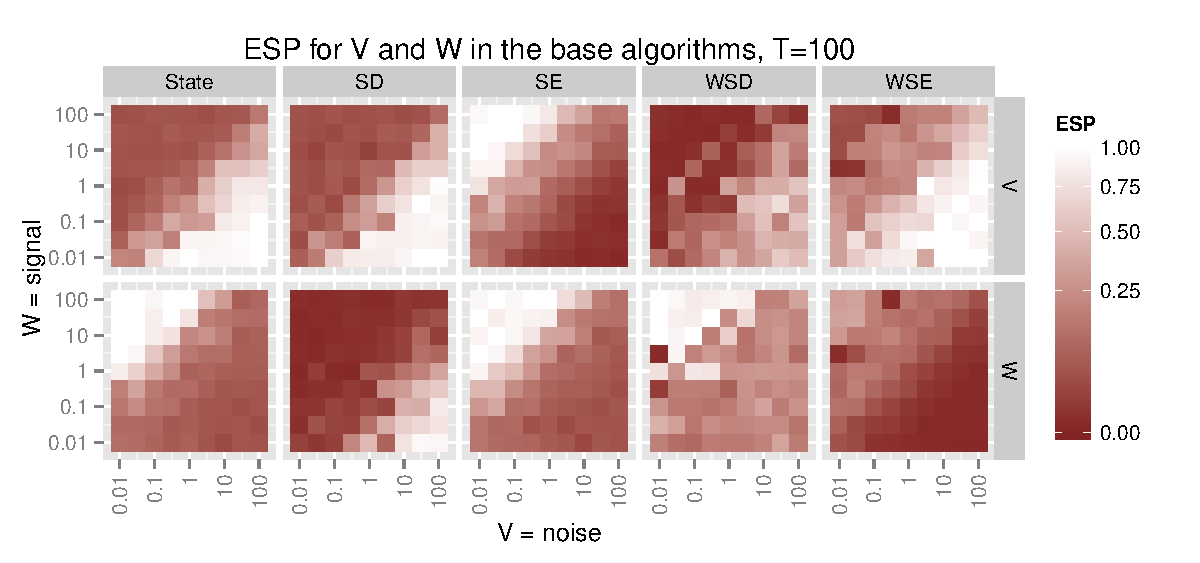
\includegraphics[width=0.7\textwidth]{baseESplot100}
\caption{Effective sample proportion in the posterior sampler for a time series of length $T=100$, for $V$ and $W$ in the base samplers. $X$ and $Y$ axes indicate the true values of $V$ and $W$ respectively for the simulated data. Note that the signal-to-noise ratio is constant moving up any diagonal. In the upper left the signal is high, in the lower right the noise is high.}
\label{baseESplot}
\end{figure}

Figure \ref{baseESplot} contains plots of ESP for $V$ and $W$ in each chain of each base sampler for $T=100$ --- we omit the $T=10$ and $T=1000$ plots for brevity, but they can be found in the supplementary materials (Appendix \zref{sec:plots}). The State sampler has a low ESP for $V$ and a high ESP for $W$ when the true signal-to-noise ratio, $R^*=W^*/V^*$, is larger than one. In contrast, when $R^*<1$ the State sampler has a low ESP for $W$ and a high ESP for $V$. When $R^*\approx 1$, the state sampler has a modest to low ESP for both $V$ and $W$. To summarize, the state sampler has mixing issues for whichever of $V$ or $W$ is smaller. The WSD and WSE samplers are similar to the state sampler except WSD has lower ESP for $V$ and WSE has lower ESP for $W$. The SD sampler has low ESP for both $V$ and $W$ when $R^*>1$, and it is paricularly low for $W$. The SE sampler behaves almost exactly opposite ---it has low ESP for both when $R^*<1$ and in particular for $V$. We omit the results here, but as $T$ increases, in all samplers the region of the parameter space with high ESP shrinks and in the low ESP regions, ESP drops closer to zero. We summarize some of the above results for convenience in Table \ref{tab:stnmix}.
\begin{table}
  \centering
  \begin{tabular}{|l|ccccc|}\hline
    Parameter & State & SD & SEr & WSD & WSE \\\hline
    V & $R^* < 1$ & $R^* < 1$ & $R^* > 1$ & $R^* < 1$ & $R^* < 1$\\
    W & $R^* > 1$ & $R^* < 1$ & $R^* > 1$ & $R^* > 1$ & $R^* > 1$ \\\hline
  \end{tabular}
  \caption{Rule of thumb for when each base algorithm has a high ESP for each variable as a function of the true signal-to-noise ratio, $R^*=W^*/V^*$. Note that as the length of the time series increases, the farther away from one $R^*$ has to be for the sampler to have a high ESP.}
  \label{tab:stnmix}
\end{table}

Most of the patterns of Figure \ref{baseESplot} and Table \ref{tab:stnmix} can be explained by Figure \ref{corplot}, which contains the estimated posterior correlations between various functions of parameters estimated using the simulations from the Triple-Alt sampler for a time series with $T=100$. The state sampler consists of two steps --- a draw of $\theta$ given $V$ and $W$, and a draw of $(V,W)$ given $\theta$. From Section \ref{sec:LLM:fullcond} we have that conditional on $\theta$, $V$ and $W$ are independent in the posterior and each has an inverse gamma distribution that depends on the states only through the second parameter:
\begin{align*}
  b_V &= \beta_V + \sum_{t=1}^T(y_t - \theta_t)^2/2 &
  b_W &= \beta_W + \sum_{t=1}^T(\theta_t - \theta_{t-1})^2/2.
\end{align*}
So we can view $(b_V,b_W)$ as the data augmentation instead of $\theta$ and thus the state sampler is
\begin{align*}
  [b_V, b_W|V^{(k)},W^{(k)}] \to [V^{(k+1)},W^{(k+1)}|b_V,b_W].
\end{align*}
Thus the dependence between $(V,W)$ and $(b_V,b_W)$ in the posterior will determine how much the state sampler moves in a given iteration and, in particular, it is possible that $V$ and $W$ have very different serial dependence from each other since we are drawing them jointly. When the dependence between $V$ and $b_V$ is high, the $(V,W)$ step will hardly move $V$ even if it drastically moves $W$ since $V$ and $W$ are independent. However, the $(b_V,b_W)$ step may move both elements a moderate amount since they both depend on $(V,W)$.

In Figure \ref{corplot} we see that the posterior correlation between $V$ and $b_V$ is high in magnitude and positive when $R^*>1$ while the posterior correlation between $V$ and $b_W$ is moderate to low and negative. When $R^*$ is large enough though, the posterior correlation between $V$ and $b_W$ evaporates. Similarly when $R^*<1$ the posterior correlation between $W$ and $b_W$ is high and positive and the posterior correlation between $W$ and $b_V$ is high and negative. Again as $R^*$ becomes large enough the correlation between $W$ and $b_V$ goes to zero. So when $R^*>1$, the draw of $(b_V, b_W)$ is unlikely to move $b_V$ much since $b_V$ is so highly correlated with $V$ and essentially uncorrelated with $b_W$, but $b_W$ is essentially uncorrelated with $W$ and negatively correlated with $V$ so $b_W$ is likely to move a fair amount. Furthermore the draw of $V$ is highly correlated with $b_V$ while the draw of $W$ is essentially independent of $b_W$ (and the draws of $V$ and $W$ are independent conditional on $b_V$ and $b_W$). Thus when $R^*>1$ we should expect high serial dependence for $V$ and low serial dependence for $W$, and so low ESP for $V$ and high ESP for $W$, which is exactly what we see in Figure \ref{baseESplot}. By similar reasoning when $R^*<1$, we should expect low serial dependence for $V$ and high serial dependece for $W$ and thus high ESP for $V$ and low ESP for $W$, which can also be seen in Figure \ref{baseESplot}.

For the SD sampler, things are a bit more complicated. The draw of $V|W,\gamma$ still depends on $b_V$ since it is the same inverse gamma draw as in the state sampler, but the draw of $W|V,\gamma$ now depends on $a_\gamma$ and $b_\gamma$ defined in Section \ref{sec:LLM:fullcond} as 
\begin{align*}
  a_\gamma & = \frac{1}{2V}\sum_{t=1}^T\left(\sum_{j=1}^t\gamma_j\right)^2&
  b_\gamma &= \frac{1}{V}\sum_{t=1}^T(y_t-\gamma_0)\left(\sum_{j=1}^t\gamma_j\right).
\end{align*}
So the dependence between $V$ and $b_V$ determines how much the chain moves in the $V$ step, and the dependence between $W$ and $(a_\gamma , b_\gamma)$ determines how much it moves in the $W$ step. The dependence between $(V,W)$ and $\gamma$ determines how much the chain moves in the DA step, but we can view this step instead as a draw of $b_V$ in which case the dependence between $W$ and $b_V$ determines how much the chain moves in that step. So if any one of these steps has high dependence, we should expect every element of the chain, and $(V,W)$ in particular, to have high serial dependence in the chain. The SE sampler is analogous to the SD sampler except with $b_W$, $a_\psi$ and $b_\psi$ where
\begin{align*}
  a_\psi&=\frac{1}{2W}\sum_{t=1}^T(L\psi_t)^2&
  b_\psi&=\frac{1}{W}\sum_{t=1}^T(L\psi_tLy_t).
\end{align*}

\begin{figure}[!ht]
\centering
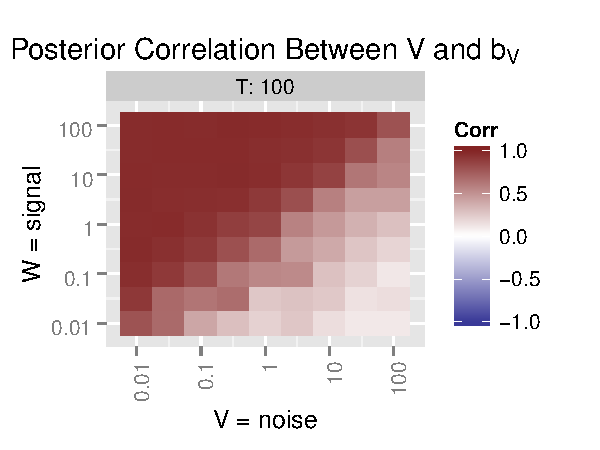
\includegraphics[width=0.24\textwidth]{corplot1}
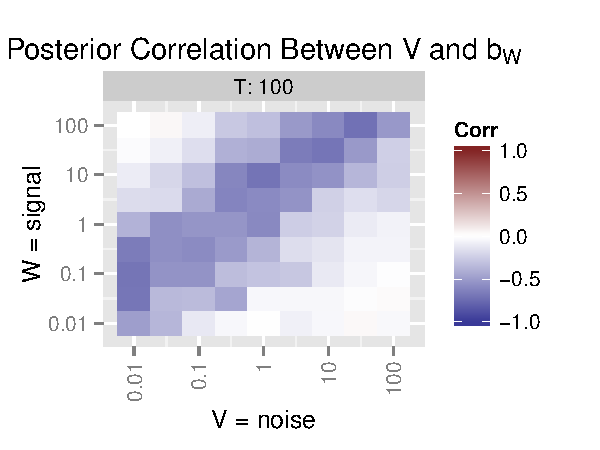
\includegraphics[width=0.24\textwidth]{corplot2}
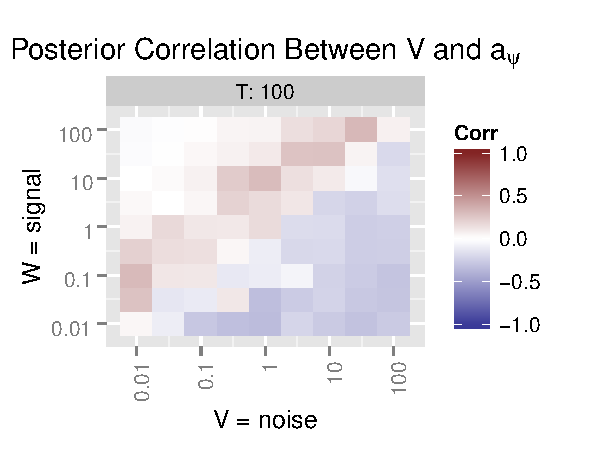
\includegraphics[width=0.24\textwidth]{corplot3}
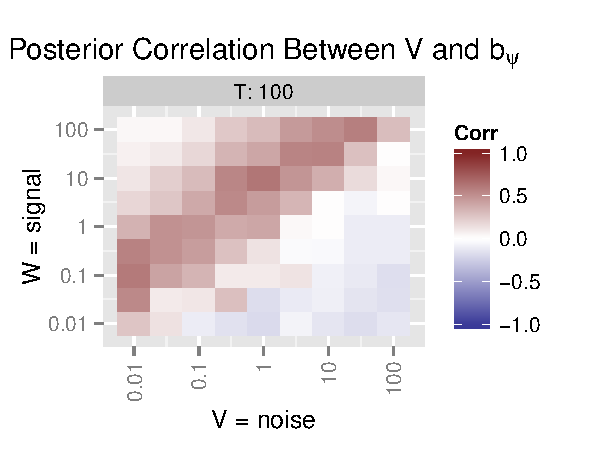
\includegraphics[width=0.24\textwidth]{corplot4}
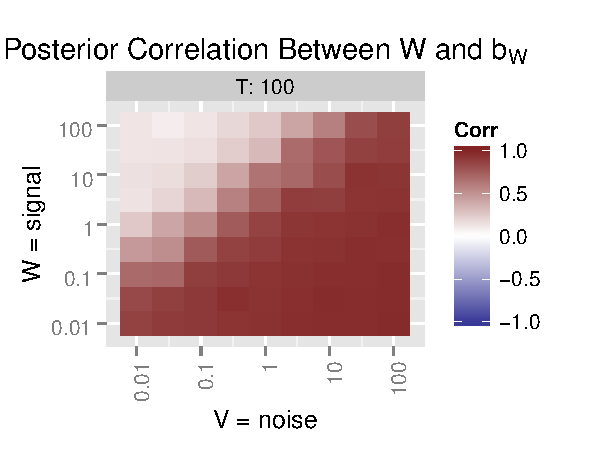
\includegraphics[width=0.24\textwidth]{corplot5}
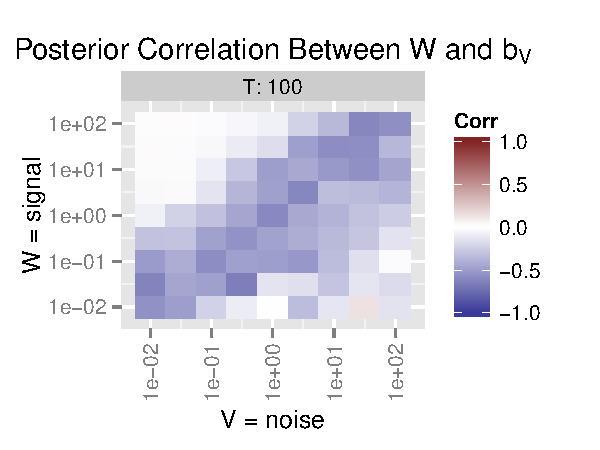
\includegraphics[width=0.24\textwidth]{corplot6}
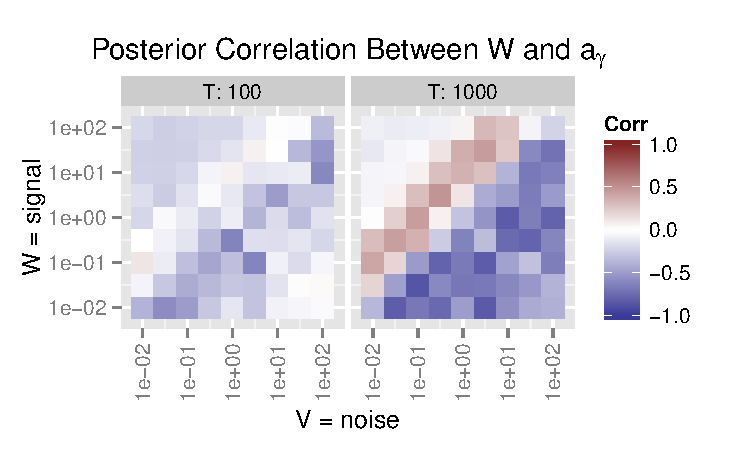
\includegraphics[width=0.24\textwidth]{corplot7}
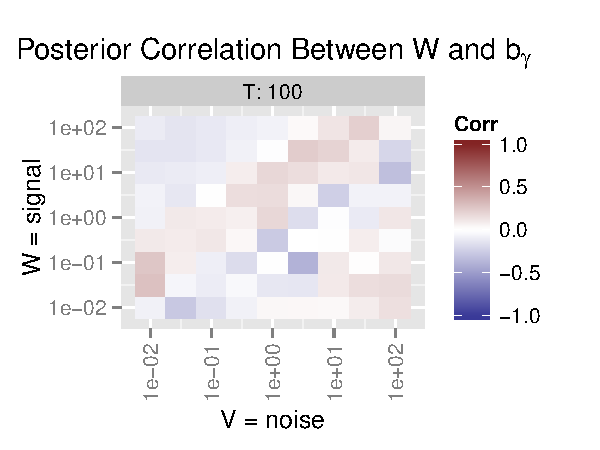
\includegraphics[width=0.24\textwidth]{corplot8}
\caption{Posterior correlation between $V$ or $W$ and $b_V$, $b_W$, $a_\gamma$, $b_\gamma$, $a_\psi$ or $b_\psi$. $X$ and $Y$ axes indicate the true values of $V$ and $W$ respectively for the simulated data with $T=100$.}
\label{corplot}
\end{figure}

In order to analyze the SD sampler, first suppose $R^*>1$. Then from Figure \ref{corplot} $b_V$ has high correlation with $V$ and low correlation with $W$, so the draw of $b_V$ should not move the chain much. Next, the draw of $V$ should again not move the chain much because of the high correlation between $V$ and $b_V$. Finally the draw of $W$ has a fair chance to move the chain because it has low correlation with both $a_\gamma$ and $b_\gamma$. But this has little impact on $b_V$ and thus the entire chain since $b_V$ is so highly correlated with $V$ but hardly correlated with $W$. So when $R^*>1$, we should expect high serial dependence and low ESP for $V$. We should also expect similar behavior for $W$ since the entire chain is hardly moving so $W$'s hyperparameters are hardly moving. This is roughly what we see in Figure \ref{baseESplot}, though this reasoning does not allow us to predict which of $V$ and $W$ will have lower ESP. When $R^*<1$ the posterior correlation in each of the steps is broken, though in the $W$ step the correlation between $W$ and both $a_\gamma$ and $b_\gamma$ becomes negative and somewhat high in magnitude. Here we should not expect less serial dependence in $V$ or $W$, but we should perhaps expect higher ESP's since negatively correlated draws decrease Monte Carlo standard error. Indeed, we see ESP's near one for both variances in Figure \ref{baseESplot}. The SE sampler is analogous to the SD sampler and a similar analysis applies --- the posterior correlations between $V$ or $W$ and $b_W$, $a_\psi$ or $b_\psi$ in Figure \ref{corplot} roughly predict the ESP of the SE sampler in Figure \ref{baseESplot}. When one or more of the correlations are high, ESPs for $V$ and $W$ are low while when all of the correlations are low, both ESPs are high. We omit a similar analysis of the wrongly-scaled samplers for brevity, but note that their behavior will allows us to predict the behavior of the CIS sampler.

\subsection{GIS and CIS Results}

We fit the LLM to the simulated datasets using several GIS samplers and a CIS sampler as well. Since the wrongly-scaled samplers behaved similarly to the state sampler and neither of the underlying DAs were a SA for $V$ and $W$ jointly, we ignored them in the construction of the GIS samplers. Instead, we constructed the State-SD, State-SE, SD-SE, and Triple (State-SD-SE) GIS samplers, as well as the CIS sampler.

Based on the intuition in Section \ref{sec:Intro:int}, both the GIS and Alt algorithms should work best when at least one of the underlying base algorithms has a high ESP. This suggests that the SD-SE algorithms will have the best performance for both $V$ and $W$ of the GIS and Alt algorithms which use two DAs, especially when $R^*$ is far away from one. However, when $R^*$ is near one they may offer no improvement over the State sampler, especially for large $T$. We showed in Section \ref{sec:Algs:CIS} that the CIS and the SD-SE GIS algorithm consist of the same steps, just rearranged. This suggests that they should perform similarly so that we expect the CIS algorithm to have good mixing for both $V$ and $W$ when $R^*$ is sufficiently different from one. 

\begin{figure}[!ht]
\centering
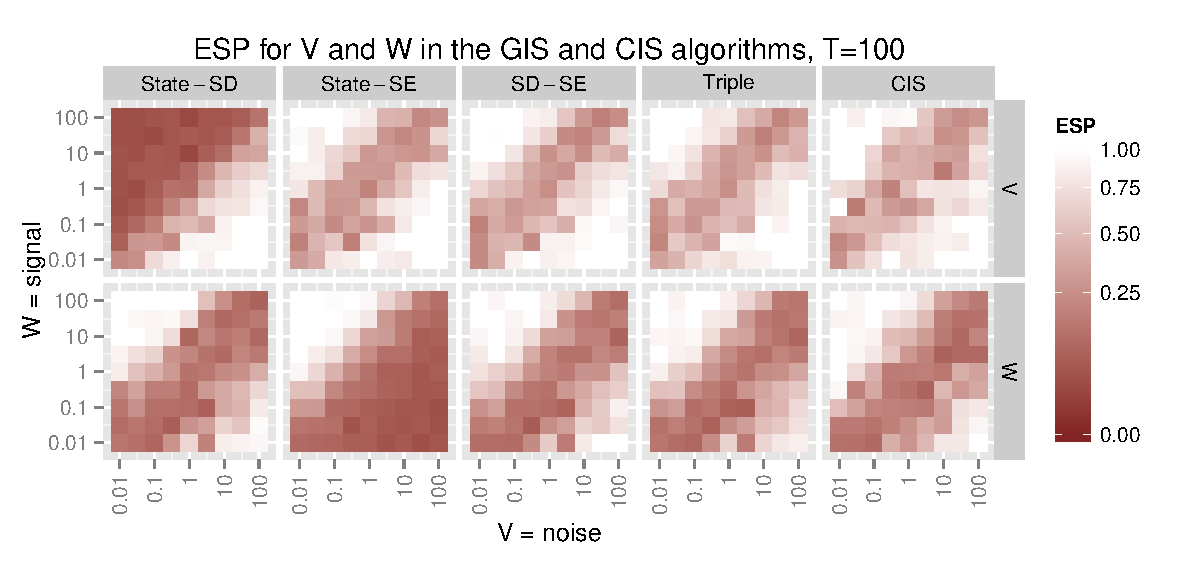
\includegraphics[width=0.7\textwidth]{intESplot100}
\caption{ESP in the posterior sampler for $V$ and $W$ in for $T=100$ in all four GIS samplers based on any two or three of the states, scaled disturbances and scaled errors as well as the CIS sampler.}
\label{intESplot}
\end{figure}

We can verify most of these intuitions in Figure \ref{intESplot}. First, the State-SD GIS algorithm has high ESP for $W$ except for a narrow band where $R^*$ is near one. The State-SD GIS algorithm's mixing behavior for $V$ appears identical to the original State sampler --- high ESP when $R^* < 1$ and poor ESP when $R^* > 1$. So this algorithm behaves as expected --- it takes advantage of the fact that the state and SD DA algorithms make up a ``beauty and the beast'' pair for $W$ and thus improves mixing in the marginal chain for $W$. However, the two underlying DA algorithms behave essentially identically for $V$ so there is no improvement in that marginal chain. Similarly the State-SE GIS algorithm's ESP for $W$ is essentially identical to the State and SE algorithms' ESP for $W$ --- high when $R^*$ large and low when $R^*$ small. For $V$, the State-SE algorithm has a high ESP when $R^*$ is far enough away from one, especially when $T$ is small. The SD-SE GIS algorithm also behaves as predicted --- when $R^*$ is not too close to one it has high ESP for both $V$ and $W$, though it has extra trouble with $W$ when $R^*$ is less than one but not small enough. The SD-SE GIS algorithm behaves apparently identically to the CIS and Triple GIS algorithms. The first of these is not surprising --- based on the intuition that the SD-SE GIS and CIS algorithms are the same up to a reordering of each of their steps, we expected little if any difference. However, we had some hope that the Triple GIS algorithm would improve upon the SD-SE GIS algorithm somewhat by further breaking the correlation between iterations in the Markov chain. 

\begin{figure}[!ht]
\centering
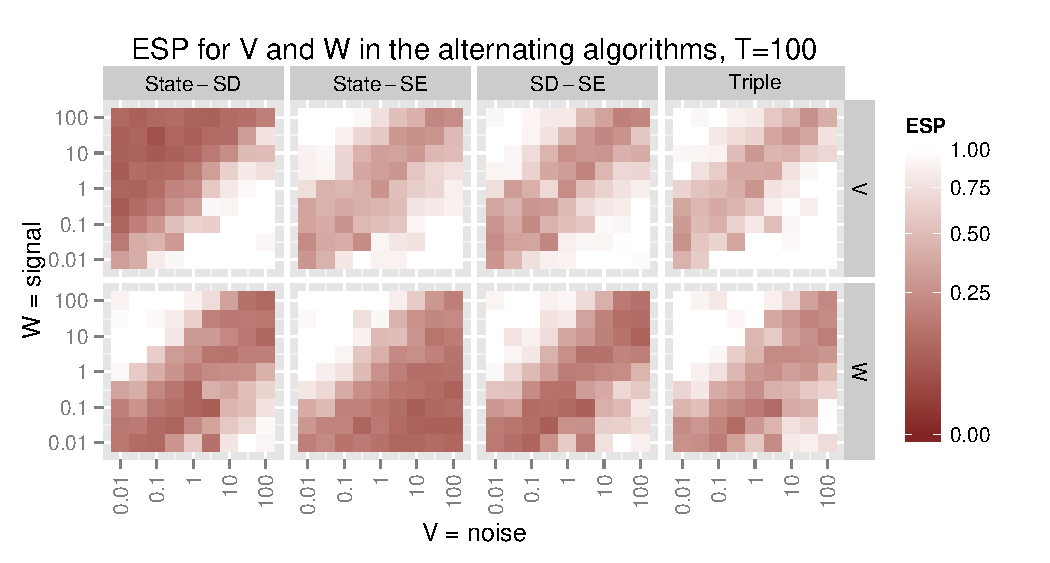
\includegraphics[width=0.7\textwidth]{altESplot100}
\caption{ESP in the posterior sampler for $V$ and $W$ for $T=100$ in all four alternating samplers based on any two or three of the states, scaled disturbances and scaled errors.}
\label{altESplot}
\end{figure}


We also fit each Alt sampler that corresponds to one of the GIS samplers we fit, that is the State-SD, State-SE, SD-SE and Triple (State-SD-SE) Alt samplers. Figure \ref{altESplot} contains the ESP of these samplers for both $V$ and $W$. There appears to be little practical difference between the alternating and interweaving versions of a given algorithm based on any two or three of the base DAs --- both take advantage of the beauty and the beast nature of their underlying DAs, but apparently dependence between the two DAs prevents the GIS version of the sampler from improving on the Alt version. All of these results are summarized in Table \ref{tab:stnmix2}. We include simulations with differing sizes of $T$ using these samplers in the supplementary materials (Appendix \zref{sec:plots}), but the upshot is that, like with the base samplers, increasing the length of the time series worsens ESP for both $V$ and $W$ in all samplers and in particular shrinks the area of the parameter space in which ESP is high.

\begin{table}
  \centering
  \begin{tabular}{|l|ccccc|}\hline
    Parameter & State-SD        & State-SE       & SD-SE        & Triple            & Full CIS \\\hline
    V         & $R^* < 1$           & $R^* \not\approx 1$ & $R^* \not\approx 1$ & $R^* \not\approx 1$ & $R^* \not\approx 1$ \\
    W         & $R^* \not\approx 1$ & $R^* > 1$           & $R^* \not\approx 1$ & $R^* \not\approx 1$ & $R^* \not\approx 1$\\\hline
  \end{tabular}
  \caption{Rule of thumb for when each interweaving or alternating algorithm has a high ESP for each variable as a function of the true signal-to-noise ratio, $R^*=W^*/V^*$. Note that as the length of the time series increases, the farther away from one $R^*$ has to be for the sampler to have a high ESP.}
  \label{tab:stnmix2}
\end{table}

\subsection{Computational time}\label{sec:LLM:time}

From a practical standpoint a more important question than how well the chain mixes is the full computational time required to adequately characterize the target posterior distribution. In order to investigate this, we compute the natural log of the average time in minutes required for each sampler to achieve an effective sample size of 1000 --- in other words the log minutes per 1000 effective draws. All simulations were performed on a university cluster with Intel Xeon X5675 3.07 GHz processors. While different systems will yield different absolute times, the relative times should at least be similar. Figure \ref{baseinttimeplot} contains plots of the log minutes per 1000 effective draws for both $V$ and $W$ and for each of the base and interweaving samplers.

For $T=100$ we see that the pattern we saw for ESP also appears for log minutes per 1000 effective draws. The State sampler becomes slow to reach 1000 effective draws for $V$ when $R^*>1$ and for $W$ when $R^*<1$. The SD and SE samplers behave as expected --- the SD sampler is slow for both $V$ and $W$ when $R^*>1$ while the SD sampler is slow for both $V$ and $W$ when $R^*<1$. The SD-SE GIS, Triple GIS and Full CIS algorithms appear to be the big winners here and are almost indistinguishable. All three algorithms are slightly slower for both $V$ and $W$ when $R^*$ is near one, though for larger $T$,  when $R^*$ is near or below one all three are slow for $W$ (plots available in Appendix \zref{sec:plots} of the supplementary materials). Compared to the state sampler though, all three offer large gains over most of the parameter space. Figure \ref{altinttimeplot} shows the log time per 1000 effective draws for the Alt algorithms and we see essentially the same pattern as we saw for the GIS algorithms, so there is no clear advantage to using the alternating or interweaving version of any algorithm.


\begin{figure}[!ht]
\centering
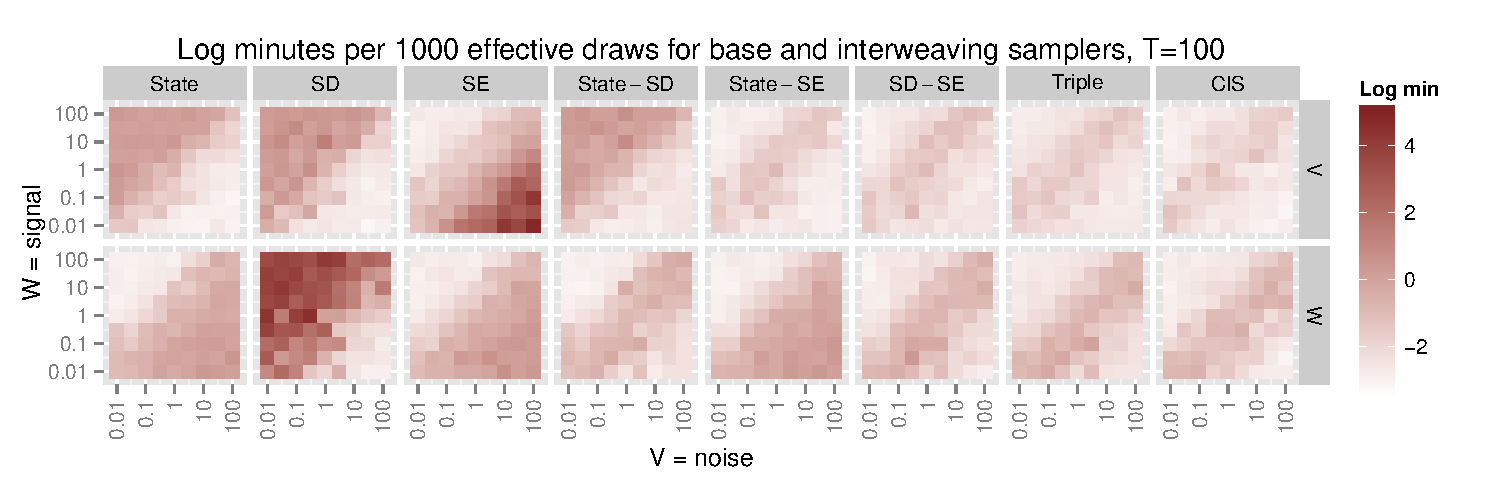
\includegraphics[width=0.8\textwidth]{baseinttimeplot100}
\caption{Log of the time in minutes per 1000 effective draws in the posterior sampler for $V$ and $W$, for $T=100$ in the state, scaled disturbance and scaled error samplers and for all five interweaving samplers.}
\label{baseinttimeplot}
\end{figure}


\begin{figure}[!ht]
\centering
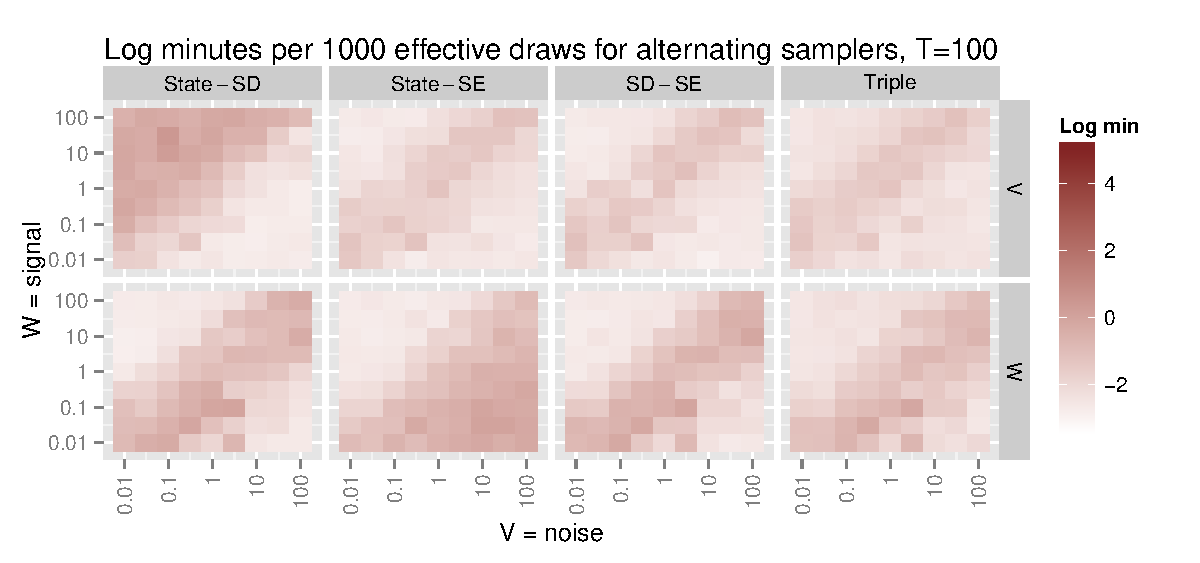
\includegraphics[width=0.7\textwidth]{altinttimeplot100}
\caption{Log of the time in minutes per 1000 effective draws in the posterior sampler for $V$ and $W$, for $T=100$ in the alternating samplers.}
\label{altinttimeplot}
\end{figure}

\section{Discussion}\label{sec:Discuss}

The importance of reparameterization in DA algorithms is well known \cite{papaspiliopoulos2007general}, both in term of reparameterizing the model parameters and reparameterizing the DA. In order explore reparameterizing the DA in dynamic linear models, we start with two DAs --- the usual DA, called the latent states, and the scaled disturbances, often called the noncentered disturbances, obtained by centering and scaling the latent states appropriately. In addition, we introduce three new DAs for the DLM, the scaled errors, the wrongly-scaled disturbances, and the wrongly-scaled errors, all obtained by an analogy with the scaled disturbances. We introduce these DAs for the purpose of applying the interweaving strategies of \citeasnoun{yu2011center}. In particular we apply GIS, obtained by interweaving between two separate DAs, and CIS, obtained by applying GIS in separate Gibbs steps to sub-blocks of the parameter vector. We also seek to apply ASIS, which is a GIS where the two DAs are required to be a sufficient augmentation and an ancillary augmentation. However, we find that under reasonable assumptions that any sufficient augmentation for the general DLM yields a full conditional distribution for the model parameters that is as difficult to sample from as the target posterior distribution of the model parameters. So ASIS probably is not a fruitful sampling strategy in the DLM, though perhaps with some creativity a suitable SA can be found.

With the DAs we do have available to us, we construct each possible DA algorithm, several GIS algorithms and their corresponding Alt algorithms, and a CIS algorithm for the general DLM. The full conditional posterior of the model parameters given any of the scaled DAs turns out to be complicated and difficult to sample from. As a result, we are forced to draw the system variance and observation variance in two steps instead of one. One of the these two draws is still difficult, but at least in the local level model it is manageable. Using the local level model as an example, we explored the mixing properties of many of the available DA, GIS, Alt, and CIS algorithms by fitting the model to simulated datasets. We find that the true signal-to-noise ratio, $R^*=V^*/W^*$, is important for determining when each algorithm performs well, and in addition that there appears to be no substantive difference between a GIS algorithm an its corresponding Alt algorithm. In fact, the three best performing algorithms under most circumstances are the SD-SE GIS algorithm, the SD-SE Alt algorithm and the CIS algorithm. In some regions of the parameter space, all three algorithms are substantially faster than the commonly used State sampler.

Some of our results have been anticipated in the literature, in particular the importance of the true signal-to-noise ratio to the mixing and convergence properties of various MCMC algorithms. In the AR(1) plus noise model, \citeasnoun{pitt1999analytic} find that the signal-to-noise ratio along with the AR(1) coefficient determine the convergence rate of a Gibbs sampler. In addition, they find that as the length of the time series increases the convergence rate decreases, which is consistent with our empirical findings in the local level model. When \citeasnoun{fruhwirth2004efficient} study the dynamic regression model with a stationary AR(1) process on the regression coefficient, they use both the states and the scaled disturbances (in their language, the noncentered disturbances) and several other DAs motivated by some results for Gibbs samplers in the hierarchical model literature. When they examine the behavior of the resulting DA algorithms, \citeasnoun{fruhwirth2004efficient} find that the relative behavior of the SD sampler and the State sampler depends on a function of the true signal-to-noise ratio that also depends on the true value of the autocorrelation parameter and the distribution of the covariate. In addition none of the other DA algorithms they consider are more efficient than both the state sampler and the SD sampler. This holds true both when they assume that the autorcorrelation parameter is known and when it is assumed unknown and must be estimated. Their result is encouraging since the extra complexity from adding a new parameter to the model could change the properties of the DA algorithms based on an AA, but it appears the differences are relatively small.

While it is clear that the signal-to-noise ratio is the key quantity for determining how well one of MCMC algorithms we discussed will perform in the local level model, in the general DLM we do not know whether the signal-to-noise ratio has any relevance. However, given the results of previous work discussed above it is likely that the signal-to-noise ratio will in some way determine how well each algorithm performs. The precise manner in which convergence and mixing behavior depends on the true signal-to-noise ratio is unkown, but it is likely a consequence of the relevance of the Bayesian fraction of missing information and the related EM fraction of missing information to the performance of the DA and EM algorithms (see \citeasnoun{van2001art} for a good explication of both concepts).


\subsection{Improving computational efficiency}

A major computational bottleneck in most of our algorithms occurs when we have to draw from $p(W|V,\gamma,y)$, $p(V|W,\psi,y)$, $p(V|W,\tilde{\gamma},y)$ or $p(W|V,\tilde{\psi},y)$. The densities $p(W|V,\gamma,y)$ and $p(V|W,\psi,y)$ have the form
\[
p(x)\propto x^{-\alpha-1}\exp\left[-ax + b\sqrt{x} - c/x\right],
\]
while the densities $p(W|V,\tilde{\psi},y)$ and $p(V|W,\tilde{\gamma},y)$ have the form
\[
p(x)\propto x^{-\alpha-1}\exp\left[ -ax + b/\sqrt{x} -c/x\right]
\]
where $\alpha,a,c>0$ and $b\in\Re$. When $b=0$ we have a special case of the generalized inverse Gaussian (GIG) distribution, so perhaps the methods used to speed up draws from the GIG can be used here \cite{jorgensen1982statistical,dagpunar1989easily,devroye2012random}. On the other hand, it might be worth putting effort into drawing $V$ and $W$ jointly conditional on the (wrongly) scaled disturbances or the (wrongly) scaled errors. Using the scaled disturbances, the conditional distribution of $V$ given $W$ is inverse gamma in the LLM and inverse Wishart in the general DLM, so it is easy to derive the marginal density $p(W|\gamma,y)$ up to a proportionality constant. In our LLM example, this density turns out to be very difficult to sample from and, in particular, it is not easy to come up with a generally good approximation for rejection sampling or for a Metropolis step. 

The main problem is that the augmented data likelihood and the prior for the variance we used to scale the states combine to create a complicated full conditional for that variance, e.g. $p(y,\gamma|V,W)$ and $p(W)$, combine to create a complicated full conditional for $W$. We initially chose inverse Wishart priors for $V$ and $W$ partially because they are standard and partially for computational convenience, i.e. they are conditional conjugate with the states which results in full Gibbs steps in the state sampler. But in this case, there may be a more convenient prior. In addition, there are well known inferential problems with the inverse Wishart prior in the hierarchical model literature, e.g. \citeasnoun{gelman2006prior} and \citeasnoun{alvarez2014cov}, though it is unclear whether this transfers over to DLMs or more generally any time series model. An alternative is to use the conditionally conjugate prior conditional on the scaled disturbances, or whichever DA we prefer.

In the LLM, the conditionally conjugate prior for $\sqrt{W}$ using the scaled disturbances as the DA is a Gaussian distribution --- strictly speaking this prior is on $\pm \sqrt{W}$. If we use this prior for $\pm\sqrt{V}$ as well, the $V$ step in the scaled disturbance sampler becomes a draw from the generalized inverse Gaussian distribution. This prior has been used by \citeasnoun{fruhwirth2011bayesian} and \citeasnoun{fruhwirth2008bayesian} to speed up computation while using the scaled disturbances in hierarchical models and by \citeasnoun{fruhwirth2010stochastic} for time series models with a DA similar to the scaled disturbances (the latent states are scaled, but not centered). We omit the results here, but using this prior on both variances does not alter our mixing results for any of the MCMC samplers --- effective sample sizes were basically the same with either prior. There is a trade-off in computation time to consider, however. For example when using the scaled disturbances, the draw of $W|V,\gamma,y$ is sped up by using the Gaussian prior on $\pm\sqrt{W}$ since it becomes a Gaussian draw while the $V|W,\gamma,y$ is slower since it becomes a generalized inverse Gaussian draw instead of an inverse gamma. The gains outweigh the costs, at least in the local level model.

In the general DLM, however, it is unclear whether this will hold. In particular in the scaled disturbance sampler, when $V$ is a matrix its full conditional becomes a matrix analogue of the generalized inverse Gaussian distribution while when $W$ is a matrix, the nonzero elements of the Cholesky decomposition of $W$ now how the Gaussian prior and Gaussian full conditional posterior. The former is likely difficult to draw from efficiently and the latter requires additional matrix computations during every iteration. On the other hand with the inverse Wishart priors, when $W$ is a matrix the full conditional of $W$ becomes a matrix analogue of the density in Section \ref{sec:LLM:fullcond}, and this is more complicated than the matrix analogue of the GIG distribution.


\section{Supplementary Materials}

Appendices: This file provides 6 appendices cited in the main article:

\begin{itemize}
\item[] Appendix \zref{sec:DLMfullcond}: Derivations of joint distributions and full conditional distributions for each DA in the DLM.
\item[] Appendix \zref{sec:MCFA}: Mixed Cholesky factorization algorithm (MCFA) for simulation smoothing.
\item[] Appendix \zref{sec:F}: Further augmentation for non-invertible $F_t$.
\item[] Appendix \zref{sec:scaledraw}: Efficiently drawing from $p(W|V,\gamma,y)$ and $p(V|W,\psi,y)$ in the LLM.
\item[] Appendix \zref{sec:wscale}: Efficiently drawing from $p(W|V,\tilde{\gamma},y)$ and $p(V|W,\tilde{\psi},y)$ in the LLM.
\item[] Appendix \zref{sec:plots}: Further plots of ESP and computational time for different values of $T$.
\end{itemize}

Code: This file contains code for obtaining the simulations used in the LLM example from Section \ref{sec:LLM} and, in particular, for the MCFA and each MCMC algorithm for the LLM.

\clearpage
\bibliographystyle{ECA_jasa}  % proper bibliography style for ASA
\bibliography{dlmasis}
\end{document}

